\documentclass[%
 onecolumn,
 amsmath,amssymb,
 aps,
 prl,
 nofootinbib,nobibnotes,
]{revtex4-2}

% \bibliographystyle{apsrev4-1}

% \usepackage{widetext}
\usepackage{graphicx}
\usepackage{tabularx}
\usepackage{dcolumn}
\usepackage{bm}
\usepackage{bold-extra}
\usepackage[ruled,vlined]{algorithm2e}

\usepackage[dvipsnames]{xcolor}
\usepackage[hidelinks]{hyperref}
\usepackage{acronym}
\usepackage{physics}
\usepackage{orcidlink}
\usepackage{xspace}
\usepackage{datatool}

\graphicspath{{plots}{plots/posterior_samples}{plots/prior_samples}}


\newacro{PE}[PE]{parameter estimation}
\newacro{GW}[GW]{gravitational-wave}
\newacro{GWTC-5}[GWTC-5]{fifth gravitational-wave transient catalog}
\newacro{GWTC-4}[GWTC-4]{fourth gravitational-wave transient catalog}
\newacro{GWTC-3}[GWTC-3]{third gravitational-wave transient catalog}
\newacro{GWTC-2}[GWTC-2]{second gravitational-wave transient catalog}
\newacro{GWTC}[GWTC]{gravitational wave transient catalog}
\newacro{LVK}[LVK]{LIGO---Virgo---KAGRA collaborations}
\newacro{O4}[O4]{fourth observing run}
\newacro{O3}[O3]{third observing run}
\newacro{HMC}[HMC]{Hamiltonian Monte Carlo}
\newacro{MC}[MC]{Monte Carlo}
\newacro{NUTS}[NUTS]{No-U-Turn Sampler}
\newacro{IID}[IID]{identically and independently distributed}
\newacro{SFR}[SFR]{star formation rate}
\newacro{KDE}[KDE]{kernel density estimate}
\newacro{BBH}[BBH]{binary black-hole}
\newacro{BNS}[BNS]{binary neutron star}
\newacro{NSBH}[NSBH]{neutron star-black hole binary}
\newacro{NS}[NS]{neutron star}
\newacro{BH}[BH]{black hole}
\newacro{GR}[GR]{general relativity}


\newacro{PISN}[PISN]{pair-instability supernova}
\newacro{PPISN}[PPISN]{pulsational pair-instability supernova}    



\newacro{PPC}[PPC]{posterior predictive check}
\newacro{MI}[MI]{mutual information}
\newacro{CAR}[CAR]{conditional autoregressive}
\newacro{ICAR}[ICAR]{intrinsic conditional autoregressive}
\newacro{PDF}[PDF]{probability density function}
\newacro{KL}[KL]{Kullback--Leibler}
\newacro{JS}[JS]{Jensen--Shannon}

\newacro{XLA}[XLA]{Accelerated Linear Algebra}
\newacro{HLV}[HLV]{Hanford, Livingston and Virgo}
\newacro{FAR}[FAR]{false-alarm rate}
\newacro{SNR}[SNR]{signal-to-noise ratio}
\newacro{IID}[IID]{independent and identically distributed}
\newacro{PSD}[PSD]{power spectral density}
\newacro{DAG}[DAG]{directed acyclic graph}


% 
% Channels
%
\newacro{CE}[CE]{common-envelope}
\newacro{OC}[OC]{open cluster}
\newacro{NSC}[NSC]{nuclear star cluster}
\newacro{CHE}[CHE]{chemically-homogeneous evolution}
\newacro{GC}[GC]{globular cluster}
\newacro{AGN}[AGN]{active galactic nuclei}
\newacro{SMT}[SMT]{stable mass transfer}

\newacro{MS}[MS]{main sequence}
\newacro{SN}[SN]{supernova}
\newacroplural{SN}[SNe]{supernovae}
\newacro{XRB}[XRB]{X-ray binary}
\newacroplural{XRB}[XRBs]{X-ray binaries}



\newacro{CAR}[CAR]{conditional auto-regressive}
\newacro{SPDE}[SPDE]{stochastic partial differential equation}
\newacro{GMRF}[GMRF]{Gaussian Markov random field}


% numbers: copies of ../macros/*.tex (notebooks/draft_figures.sh macros); use in math mode, e.g. $\peakTenMuFlex\,\Msun$.
% Found from draft/ or from the repository root.
\newcommand{\inputmacros}[1]{\IfFileExists{macros/#1.tex}{\input{macros/#1}}{\input{draft/macros/#1}}}
\inputmacros{peak_fits}
\inputmacros{joint_fits}
\inputmacros{peak_pairs}
\inputmacros{peak_excess}
\inputmacros{q_contrast}
\inputmacros{peak_odds}
\inputmacros{chi_q_broadening}
\inputmacros{peak_spins}

% math macros
\newcommand{\Msun}{\ensuremath{\mathrm{M}_{\odot}}}
\newcommand{\chieff}{\ensuremath{\chi_{\mathrm{eff}}}}
\newcommand{\chip}{\ensuremath{\chi_{\mathrm{p}}}}
\newcommand{\mchirp}{\ensuremath{\mathcal{M}_c}}
\newcommand{\peryear}{\ensuremath{\,\mathrm{yr}^{-1}}}

\newcommand{\red}[1]{{\color{Red} #1}}
\newcommand{\todo}[1]{{\color{Blue}\bf TODO: #1}}
\newcommand{\jh}[1]{{\color{orange}JH: #1}}
\newcommand{\comment}[1]{}
\newcommand{\PixelPop}{\textsc{PixelPop}\xspace}
\newcommand{\gwpopulation}{\textsc{GWPopulation}\xspace}
\newcommand{\BrokenPowerlawTwoPeaks}{\textsc{Broken Powerlaw Plus Two Peaks}\xspace}
\newcommand{\flexiblespins}{\textsc{Flexible}\xspace}
\newcommand{\gaussianspins}{\textsc{Gaussian}\xspace}
% feature labels: approximate measured locations (m1 in Msun); macro names keep the old round numbers
\newcommand{\featTen}{10\xspace}
\newcommand{\featTwenty}{21\xspace}
\newcommand{\featThirtyFive}{33\xspace}
\newcommand{\featSixty}{59\xspace}


\newcommand{\heading}[1]{\textbf{\textit{#1}}}

\newcommand{\LSE}{\operatorname{LSE}}
% Main-text float numbers are hard-coded below (letter.tex order): Fig. 1 mass, 2 spin peaks, 3 bookkeeping,
% 4 sigma(q), 5 sigma(m1), 6 additive model; Table I peaks, II spins. Update them if the letter changes.

\begin{document}

\title{Supplemental Material: Nonparametric mass and spin inference reveals peaks and correlations \jh{title sucks, tbd}}

\author{Jack Heinzel\,\orcidlink{0000-0002-5794-821X}}
\email{jheinzel@flatironinstitute.org}

\author{Matthew Mould\,\orcidlink{}}


\date{\today}



\maketitle

\setcounter{equation}{0}
\setcounter{figure}{0}
\setcounter{table}{0}
\setcounter{section}{0}
\renewcommand{\theequation}{S\arabic{equation}}
\renewcommand{\thefigure}{S\arabic{figure}}
\renewcommand{\thetable}{S\arabic{table}}
\renewcommand{\thesection}{S\arabic{section}}


This Supplemental Material describes the data (Sec.~\ref{sm: data}), the likelihood and its Monte Carlo uncertainty (Secs.~\ref{sm: likelihood} and~\ref{sm: mc}), the Mat\'ern field prior (Sec.~\ref{sm: fields}), the population models (Secs.~\ref{sm: mass model} and~\ref{sm: spin models}), their implementation and sampling (Secs.~\ref{sm: implementation} and~\ref{sm: sampling}), the post-processing into spin moments (Sec.~\ref{sm: moments}), the peak fits (Sec.~\ref{sm: peak fits}), each of the four mass features (Sec.~\ref{sm: features}), the significance of the peaks (Sec.~\ref{sm: significance}), robustness tests and model comparisons (Sec.~\ref{sm: robustness}), and the hierarchical-merger expectations used in the main text (Sec.~\ref{sm: hierarchical}).

\section{Data}
\label{sm: data}

\textit{Events.} We use the 259 \acp{BBH} with \ac{FAR} $< 1\peryear$ in the population analysis of \citet{LIGOScientific:2026ctl}, spanning the first through fourth observing runs (O1--O4b), with the same event list, exclusions and waveform choices. The \ac{PE} samples come from the GWTC-2.1 and GWTC-3 data releases for O1--O3 and from the GWTC-4 and GWTC-5 releases for O4a and O4b. For each event we take the first available of NRSur7dq4~\cite{Varma:2019csw}, the mixed-waveform samples, and IMRPhenomXPHM-SpinTaylor~\cite{Pratten:2020ceb}. The list excludes sub-threshold events and events with a possible neutron star, including GW190814 and GW190917. Each sample carries its \ac{PE} prior density, which we convert to $(\ln m_1, q, \chieff, \chip, z)$, including the Jacobians of the transformation. \todo{cite the data releases}

\textit{Sensitivity.} We estimate the selection function with the mixture of sensitivity injections released with \ac{GWTC-5}: real-noise injections for O3, O4a and O4b and semianalytic injections for O1 and O2, with the same detection threshold as the events (\ac{FAR} $< 1\peryear$, and a network signal-to-noise ratio above 10 for the semianalytic injections).

\textit{Domain.} Samples and injections are restricted to $m_1 \in [3, 200]\,\Msun$ and $z < 1.9$. Samples outside this domain are given zero weight (an infinite \ac{PE} prior), and injections outside it are removed.

\textit{Sample selection.} The number of \ac{PE} samples differs between events. We keep at most 20000 samples per event, drawn at random from the \emph{usable} samples: those inside the population grid, in a $(\ln m_1, q)$ bin and a $(\chieff, \chip)$ bin that at least one detected injection reaches. Samples that are not usable carry zero weight in the likelihood anyway, since the population density at an unreachable bin cannot be constrained by the selection function. Leaving them out of the count shifts each event's log-likelihood by the constant $-\ln(N_{\rm usable}/N_{\rm real})$, which does not affect inference. Over the catalog, a fraction $9.7 \times 10^{-4}$ of samples is not usable, at most 2.3\% for one event (GW230704, mostly at $z > 1.9$). Events with fewer samples are padded to a rectangular array with zero-weight copies, and the per-event sample count is kept for the Monte Carlo estimators below.

\section{Likelihood}
\label{sm: likelihood}

For hyperparameters $\Lambda$, we write the population as a density $p(\theta \mid \Lambda)$ over $\theta = (\ln m_1, q, \chieff, \chip, z)$ and the merger rate as $R\, p(\theta \mid \Lambda)$. Marginalizing over $R$ with a scale-invariant prior gives the standard hierarchical likelihood~\cite{Mandel:2018mve, Thrane:2018qnx}
\begin{equation}
    \ln \mathcal{L}(\Lambda) = \sum_{i=1}^{N_{\rm obs}} \ln \hat{\mathcal{L}}_i(\Lambda) - N_{\rm obs} \ln \hat{\xi}(\Lambda),
\end{equation}
with the Monte Carlo estimates
\begin{equation}
    \hat{\mathcal{L}}_i = \frac{1}{M_i} \sum_{j=1}^{M_i} w_{ij}, \quad w_{ij} = \frac{p(\theta_{ij} \mid \Lambda)}{\pi_i(\theta_{ij})}, \qquad
    \hat{\xi} = \frac{1}{T} \sum_{k\,\in\,\rm found} w_k, \quad w_k = \frac{p(\theta_k \mid \Lambda)}{p_{\rm draw}(\theta_k)},
\end{equation}
where $\theta_{ij}$ are the $M_i$ samples of event $i$ with \ac{PE} prior $\pi_i$, and $\theta_k$ the found injections out of $T$ generated, with draw density $p_{\rm draw}$. Both weights include the redshift factor $\frac{dV_c}{dz} \frac{1}{1+z} (1 + z)^{\lambda}$.

\textit{Monte Carlo uncertainty.} The variance of the log-likelihood estimate is
\begin{equation}
    \sigma^2_{\ln \mathcal{L}} = \sum_i \frac{1}{N_{{\rm eff}, i}} + \frac{N_{\rm obs}^2}{N_{\rm eff, sel}}, \qquad
    N_{{\rm eff}, i} = \left[\frac{\sum_j w_{ij}^2}{(\sum_j w_{ij})^2} - \frac{1}{M_i}\right]^{-1},
\end{equation}
with the analogous effective sample size $N_{\rm eff, sel}$ for the injections~\cite{Farr:2019rap, Essick:2022ojx, Talbot:2023pex}. We record it, with its per-event and selection parts, at every posterior sample. We impose no cut on $\sigma^2_{\ln\mathcal{L}}$.

\textit{Per-event effective sample size.} Flexible models can place structure on scales smaller than an event's \ac{PE} samples resolve, where $\hat{\mathcal{L}}_i$ becomes unreliable. We therefore require $N_{{\rm eff}, i} \geq 100$ for every event, imposed as a smooth penalty, $\sum_i s(-\ln N_{{\rm eff}, i};\, -\ln 100,\, 0.1)$, where $s(x; x_0, \delta)$ is a smoothed step from zero to a large negative value at $x_0$ with width $\delta$. A smooth penalty keeps the log density differentiable for the sampler.

\textit{Selection bias correction.} $1/\hat{\xi}^{N_{\rm obs}}$ is a biased estimate of $1/\xi^{N_{\rm obs}}$. To leading order, its expectation is too large by a factor $1 + N_{\rm obs}(N_{\rm obs} + 1)\sigma_{\rm sel}^2/2$, with
\begin{equation}
    \sigma_{\rm sel}^2 = \frac{1}{T - 1}\left[T\frac{\sum_k w_k^2}{(\sum_k w_k)^2} - 1\right].
\end{equation}
Following \citet{Heinzel:2025ogf}, we subtract $N_{\rm obs}(N_{\rm obs} + 1)\sigma^2_{\rm sel}/2$ from $\ln \mathcal{L}$.

\section{Monte Carlo systematics}
\label{sm: mc}

\textit{Monte Carlo systematics.} To check that the Monte Carlo error does not drive our results, we estimate for each reported quantity $f$ the systematic shift of its posterior mean due to the Monte Carlo error of $\ln \hat{\mathcal{L}}$. To first order, the spread of this shift over Monte Carlo realizations is
\begin{equation}
    \sigma^2_{\rm syst} = \frac{1}{N^2} \sum_{n, m} \delta f_n\, \delta f_m\, C(\Lambda_n, \Lambda_m), \qquad \delta f_n = f(\Lambda_n) - \overline{f},
\end{equation}
where $C$ is the covariance of the log-likelihood error between posterior samples $\Lambda_n$ and $\Lambda_m$~\cite{Heinzel:2025ogf}. Writing $C$ as a sum over \ac{PE} samples and injections of products of normalized weights reduces this to a single pass over the posterior samples, $\sigma^2_{\rm syst} = \sum_s c_s g_s^2$ with $g_s = N^{-1}\sum_n \delta f_n \tilde{w}_{n, s}$, where $c_s = 1/[M_i(M_i - 1)]$ for the samples of event $i$ and $N_{\rm obs}^2/[T(T - 1)]$ for the injections. We compare $\sigma_{\rm syst}$ with the posterior standard deviation $\sigma_{\rm stat}$. \todo{$\sigma_{\rm syst}/\sigma_{\rm stat}$ for the peak locations, $f_{\rm ret}$ and $\sigma_{\chieff}(q)$}



We compute $\sigma_{\rm syst}$, and the precision statistic $\hat{E}$ (the information in the posterior, in bits, lost to Monte Carlo uncertainty), with \textsc{population-error}~\cite{Heinzel:2025ogf}, from the same importance weights that enter the likelihood, recomputed at every posterior sample. A quantity is robust to Monte Carlo systematics if $\sigma_{\rm syst} \ll \sigma_{\rm stat}$: the shift of its posterior mean over Monte Carlo realizations of the \ac{PE} samples and injections is then small compared with its posterior width. We evaluate this for every quantity reported in the main text: $\ln p(m_1, q)$ in each cell and the slices $p(m_1 \mid q \in Q)$, the spin moments in each $(m_1, q)$ cell and averaged over $q$ or $m_1$, the peak locations and the retained fractions. \todo{table of $\sigma_{\rm syst}/\sigma_{\rm stat}$ for these quantities and $\hat{E}$, for both spin models; state the threshold, e.g.\ $\sigma_{\rm syst}/\sigma_{\rm stat} < 0.3$}

\todo{
\begin{itemize}
    \item compute MC systematics across space
    \item run a variance cut inference (v1, v4)
    \item test weaker Neff floors
\end{itemize}
}


\section{Mat\'ern fields}
\label{sm: fields}

\IfFileExists{matern_spde.tex}{% Mat\'ern SPDE prior, adapted from J. Heinzel, \textit{An operator-based formalism for inference on the population of
% gravitational-wave sources} (LIGO DCC). Input from supplemental.tex; self-contained, so it can be dropped.
% Notation: the field amplitude is s (sigma in the DCC note), to avoid confusion with the spin widths.

All population fields are Mat\'ern Gaussian Markov random fields (\acp{GMRF}) on a regular grid. They generalize the \ac{CAR} prior of the original \PixelPop~\cite{Heinzel:2024jlc} using the correspondence between Gaussian processes and \acp{SPDE}: a foundational result~\cite{Whittle:1954abc, Whittle:1963abc, lindgren_explicit_2011} shows that the two approaches are equivalent (modulo boundary conditions), and that the Mat\'ern class of covariance kernels corresponds to the simple \ac{SPDE}
\begin{equation}
    [\kappa^2 - \nabla\cdot (H\nabla)]^{\alpha/2} \mathcal{F}(x) = \mathcal{W}(x),
    \label{eq: lrl spde}
\end{equation}
where $\mathcal{W}(x)$ is a white-noise source field, $\langle \mathcal{W}(x)\mathcal{W}(y)\rangle = \delta(x-y)$, $\alpha = D/2 + \nu$ for a Mat\'ern smoothness $\nu$ and field dimension $D$, and $H$ is a positive-definite diffusion matrix. The \ac{CAR} prior of \PixelPop is the special case $\sigma^{-1}[\kappa^2 - \nabla^2]^{1/2} \mathcal{F} = \mathcal{W}$. \acp{SPDE} are computationally efficient compared to general Gaussian process regression, which scales as $\mathcal{O}(N^3)$ in the number of latent sites, because they can exploit sparse linear algebra.

\textit{Length scales.} We take $H$ diagonal and write $H = \mathrm{diag}(\kappa^2\ell_d^2/8\nu)$, so that the \ac{SPDE} becomes
\begin{equation}
    S(\vec{\ell},\nu)\, s^{-1}\left[1 - \sum_{d=1}^D\frac{\ell_d^2}{8\nu}\partial_d^2\right]^{\alpha/2} \mathcal{F}(x) = \mathcal{W}(x),
    \label{eq: lrl spde reformated}
\end{equation}
absorbing $\kappa$ into an amplitude $s$ and introducing a scaling function $S(\vec{\ell},\nu)$ which enforces that the bin-averaged variance is exactly $s^2$ (Eq.~\ref{eq: s normalization}). With this choice, $\ell_d$ is the effective correlation range along axis $d$: \citet{lindgren_explicit_2011} found empirically that the Mat\'ern field with identity diffusion drops to $\sim 10\%$ correlation over a distance $\sqrt{8\nu}/\kappa$.

\textit{Eigenbasis.} We set Neumann (zero-derivative) boundary conditions and take the lattice to be a tensor product of one-dimensional lattices of lengths $N_1, \dots, N_D$, with basis vectors $e_{\vec{i}} = \bigotimes_{d=1}^D e_{i_d}^{(d)}$. On a uniform grid, the finite-difference Laplacian along each axis is the tridiagonal, symmetric Toeplitz matrix
\begin{equation}
    -\nabla^2 \overset{\textrm{discrete}}{\longrightarrow} \Delta \propto \begin{pmatrix}
        1 & -1 &  &  &  \\
        -1 & 2 & -1 &  &  \\
         & \ddots & \ddots & \ddots &  \\
         &  & -1 & 2 & -1  \\
         &  &  & -1 & 1
    \end{pmatrix},
    \label{eq: discrete laplacian}
\end{equation}
proportional to the univariate ICAR precision matrix used in older implementations of \PixelPop. Its eigenspectrum is analytic (the discrete cosine transform, type II)~\cite{Strang:1999dct},
\begin{equation}
    v_{k} = \sqrt{\frac{2-\delta_{k0}}{N}}\sum_{i=1}^{N} \cos\left(\frac{(2i-1)\pi k }{2N}\right) e_i, \qquad
    \lambda_k = 4\sin^2\left(\frac{\pi k}{2N}\right),
\end{equation}
for $k \in \{0, \dots, N-1\}$, with $v_k^\top v_{k'} = \delta_{kk'}$. The discretized operator of Eq.~\eqref{eq: lrl spde reformated} is then diagonal in the tensor-product basis,
\begin{equation}
    v_{\vec{k}} = \bigotimes_{d=1}^{D}v_{k_d}, \qquad
    \lambda_{\vec{k}} = s^{-1}S(\vec{\ell},\nu)\left[1 + \sum_{d=1}^D \frac{\ell_d^2}{8\nu}\lambda_{k_d}\right]^{\alpha/2},
\end{equation}
and the bin-averaged variance is $s^2$ for
\begin{equation}
    S(\vec{\ell},\nu) = \left(\frac{1}{N_{\rm tot}}\sum_{\vec{k}\neq 0}\left[1 + \sum_{d=1}^D \frac{\ell_d^2}{8\nu}\lambda_{k_d}\right]^{-\alpha}\right)^{1/2},
    \label{eq: s normalization}
\end{equation}
with $N_{\rm tot} = \prod_d N_d$. Any stationary covariance kernel with Neumann boundary conditions is diagonal under the discrete cosine transform; we restrict to the Mat\'ern class for its broad applicability and flexibility.

\textit{Sampling.} Rather than sampling the white-noise field directly, we sample in the eigenbasis of the discretized operator. The \ac{SPDE} decouples mode by mode, and because the eigenbasis is orthonormal, the projections of the discretized white noise are again independent standard normal variables. We therefore sample $z_{\vec{k}} \sim \mathcal{N}(0,1)$ for each $\vec{k}\neq 0$ and construct the field as
\begin{equation}
    \mathcal{F}(x) = \sum_{\vec{k}\neq 0} \frac{z_{\vec{k}}}{\lambda_{\vec{k}}}\, v_{\vec{k}}(x) + c_0 v_0.
    \label{eq: eigenbasis sampling}
\end{equation}
This is a non-centered parameterization~\cite{Papaspiliopoulos:2007abc, Betancourt:2017ebh}: the metaparameters $(s, \vec{\ell}, \nu)$ enter only through the eigenvalues, so the latent variables $z_{\vec{k}}$ are a priori independent of them. This avoids the funnel-shaped posteriors of a centered parameterization, in which a small $s$ or long $\ell_d$ confines the field to a narrow region and no single step size of Hamiltonian Monte Carlo is appropriate everywhere. We sample the latent coefficients, the constant mode and the metaparameters jointly with the No-U-Turn Sampler~\cite{Hoffman:2014nuts} in \textsc{NumPyro}~\cite{Phan:2019numpyro, Bingham:2019pyro}, with a dense mass matrix for the metaparameters.

\textit{The constant mode.} The $\vec{k} = 0$ eigenvector, the constant field, sets the overall offset. For a probability density, which all of our fields are, it is fixed by the normalization $\int \exp[\mathcal{F}(x)]\,dx = 1$. (For a log rate intensity, it would carry an improper uniform prior, equivalent to $\pi(R) \propto 1/R$ on the integrated rate.)

\textit{Metaparameter priors.} The diagonalized \ac{SPDE} admits any positive $\nu$, $\ell_d$ and $s$. Sensible length scales lie in $\ell_d \in [1, N_d]$ bins: over a bounded domain, $\ell_d > N_d$ has a diminishing effect on the prior. As $\nu \to \infty$ the Mat\'ern kernel approaches the radial basis function kernel, indistinguishable in practice at $\nu \gtrsim 5$, while as $\nu \to 0$ the field becomes jagged. Unless stated otherwise, we sample $\ln\nu\sim \mathcal{N}(0,0.5)$, $\ln s\sim\mathcal{N}(0,2)$ and $\ln\ell_d \sim \mathcal{U}(0,\ln N_d)$.

\textit{Boundary conditions.} Neumann boundary conditions are equivalent to an infinite Mat\'ern field with mirror-image sources at the boundaries~\cite{lindgren_explicit_2011}, so they inflate the prior variance near the edges of the domain, by up to a factor of $2^D$ at its corners.

\textit{Monte Carlo robustness.} The smoother Mat\'ern prior is more robust to Monte Carlo uncertainty in the likelihood than the \ac{CAR} prior. With a likelihood variance threshold $\sigma^2_{\ln \mathcal{L}} < 1$, the error statistic of \citet{Heinzel:2025ogf} for \ac{CAR} \PixelPop inferences is typically $\hat{E}\sim 0.2$--$0.3$ bits (that much information in the posterior is lost to Monte Carlo uncertainty), against $\hat{E}\sim 0.05$ bits for the Mat\'ern model. We expect this is because the Mat\'ern field suppresses high-frequency modes, which concentrate the population weight on a few \ac{PE} samples and injections and so reduce the effective sample sizes of the Monte Carlo integrals.

\textit{Conditional and normalized fields.} The mass field is a log density on the $(\ln m_1, q)$ grid, windowed to $m_2 > 3\,\Msun$ and normalized over the grid (Sec.~\ref{sm: mass model}). The spin fields are \textit{conditional} densities: at each $(m_1, q)$ cell, the spin field is normalized over the physical spin bins (Sec.~\ref{sm: spin models}), so any component that is constant in $(\chieff, \chip)$ cancels and is dropped. The \flexiblespins model is a single four-dimensional Mat\'ern field whose tensor-product basis is truncated to the lowest $K \times K$ modes in $(\ln m_1, q)$ and keeps all spin modes, so the conditional spin distribution varies smoothly across the mass plane and is evaluated by a contraction over mass modes without forming the four-dimensional grid (Sec.~\ref{sm: implementation}). In the \gaussianspins model, each parameter of the spin distribution is a constant plus a two-dimensional Mat\'ern field over $(\ln m_1, q)$, with the constant mode of the field set to zero so that the constant carries the mean; the additive variants replace this field by a sum of one-dimensional Mat\'ern fields, each with its constant mode set to zero.
}{% Mat\'ern SPDE prior, adapted from J. Heinzel, \textit{An operator-based formalism for inference on the population of
% gravitational-wave sources} (LIGO DCC). Input from supplemental.tex; self-contained, so it can be dropped.
% Notation: the field amplitude is s (sigma in the DCC note), to avoid confusion with the spin widths.

All population fields are Mat\'ern Gaussian Markov random fields (\acp{GMRF}) on a regular grid. They generalize the \ac{CAR} prior of the original \PixelPop~\cite{Heinzel:2024jlc} using the correspondence between Gaussian processes and \acp{SPDE}: a foundational result~\cite{Whittle:1954abc, Whittle:1963abc, lindgren_explicit_2011} shows that the two approaches are equivalent (modulo boundary conditions), and that the Mat\'ern class of covariance kernels corresponds to the simple \ac{SPDE}
\begin{equation}
    [\kappa^2 - \nabla\cdot (H\nabla)]^{\alpha/2} \mathcal{F}(x) = \mathcal{W}(x),
    \label{eq: lrl spde}
\end{equation}
where $\mathcal{W}(x)$ is a white-noise source field, $\langle \mathcal{W}(x)\mathcal{W}(y)\rangle = \delta(x-y)$, $\alpha = D/2 + \nu$ for a Mat\'ern smoothness $\nu$ and field dimension $D$, and $H$ is a positive-definite diffusion matrix. The \ac{CAR} prior of \PixelPop is the special case $\sigma^{-1}[\kappa^2 - \nabla^2]^{1/2} \mathcal{F} = \mathcal{W}$. \acp{SPDE} are computationally efficient compared to general Gaussian process regression, which scales as $\mathcal{O}(N^3)$ in the number of latent sites, because they can exploit sparse linear algebra.

\textit{Length scales.} We take $H$ diagonal and write $H = \mathrm{diag}(\kappa^2\ell_d^2/8\nu)$, so that the \ac{SPDE} becomes
\begin{equation}
    S(\vec{\ell},\nu)\, s^{-1}\left[1 - \sum_{d=1}^D\frac{\ell_d^2}{8\nu}\partial_d^2\right]^{\alpha/2} \mathcal{F}(x) = \mathcal{W}(x),
    \label{eq: lrl spde reformated}
\end{equation}
absorbing $\kappa$ into an amplitude $s$ and introducing a scaling function $S(\vec{\ell},\nu)$ which enforces that the bin-averaged variance is exactly $s^2$ (Eq.~\ref{eq: s normalization}). With this choice, $\ell_d$ is the effective correlation range along axis $d$: \citet{lindgren_explicit_2011} found empirically that the Mat\'ern field with identity diffusion drops to $\sim 10\%$ correlation over a distance $\sqrt{8\nu}/\kappa$.

\textit{Eigenbasis.} We set Neumann (zero-derivative) boundary conditions and take the lattice to be a tensor product of one-dimensional lattices of lengths $N_1, \dots, N_D$, with basis vectors $e_{\vec{i}} = \bigotimes_{d=1}^D e_{i_d}^{(d)}$. On a uniform grid, the finite-difference Laplacian along each axis is the tridiagonal, symmetric Toeplitz matrix
\begin{equation}
    -\nabla^2 \overset{\textrm{discrete}}{\longrightarrow} \Delta \propto \begin{pmatrix}
        1 & -1 &  &  &  \\
        -1 & 2 & -1 &  &  \\
         & \ddots & \ddots & \ddots &  \\
         &  & -1 & 2 & -1  \\
         &  &  & -1 & 1
    \end{pmatrix},
    \label{eq: discrete laplacian}
\end{equation}
proportional to the univariate ICAR precision matrix used in older implementations of \PixelPop. Its eigenspectrum is analytic (the discrete cosine transform, type II)~\cite{Strang:1999dct},
\begin{equation}
    v_{k} = \sqrt{\frac{2-\delta_{k0}}{N}}\sum_{i=1}^{N} \cos\left(\frac{(2i-1)\pi k }{2N}\right) e_i, \qquad
    \lambda_k = 4\sin^2\left(\frac{\pi k}{2N}\right),
\end{equation}
for $k \in \{0, \dots, N-1\}$, with $v_k^\top v_{k'} = \delta_{kk'}$. The discretized operator of Eq.~\eqref{eq: lrl spde reformated} is then diagonal in the tensor-product basis,
\begin{equation}
    v_{\vec{k}} = \bigotimes_{d=1}^{D}v_{k_d}, \qquad
    \lambda_{\vec{k}} = s^{-1}S(\vec{\ell},\nu)\left[1 + \sum_{d=1}^D \frac{\ell_d^2}{8\nu}\lambda_{k_d}\right]^{\alpha/2},
\end{equation}
and the bin-averaged variance is $s^2$ for
\begin{equation}
    S(\vec{\ell},\nu) = \left(\frac{1}{N_{\rm tot}}\sum_{\vec{k}\neq 0}\left[1 + \sum_{d=1}^D \frac{\ell_d^2}{8\nu}\lambda_{k_d}\right]^{-\alpha}\right)^{1/2},
    \label{eq: s normalization}
\end{equation}
with $N_{\rm tot} = \prod_d N_d$. Any stationary covariance kernel with Neumann boundary conditions is diagonal under the discrete cosine transform; we restrict to the Mat\'ern class for its broad applicability and flexibility.

\textit{Sampling.} Rather than sampling the white-noise field directly, we sample in the eigenbasis of the discretized operator. The \ac{SPDE} decouples mode by mode, and because the eigenbasis is orthonormal, the projections of the discretized white noise are again independent standard normal variables. We therefore sample $z_{\vec{k}} \sim \mathcal{N}(0,1)$ for each $\vec{k}\neq 0$ and construct the field as
\begin{equation}
    \mathcal{F}(x) = \sum_{\vec{k}\neq 0} \frac{z_{\vec{k}}}{\lambda_{\vec{k}}}\, v_{\vec{k}}(x) + c_0 v_0.
    \label{eq: eigenbasis sampling}
\end{equation}
This is a non-centered parameterization~\cite{Papaspiliopoulos:2007abc, Betancourt:2017ebh}: the metaparameters $(s, \vec{\ell}, \nu)$ enter only through the eigenvalues, so the latent variables $z_{\vec{k}}$ are a priori independent of them. This avoids the funnel-shaped posteriors of a centered parameterization, in which a small $s$ or long $\ell_d$ confines the field to a narrow region and no single step size of Hamiltonian Monte Carlo is appropriate everywhere. We sample the latent coefficients, the constant mode and the metaparameters jointly with the No-U-Turn Sampler~\cite{Hoffman:2014nuts} in \textsc{NumPyro}~\cite{Phan:2019numpyro, Bingham:2019pyro}, with a dense mass matrix for the metaparameters.

\textit{The constant mode.} The $\vec{k} = 0$ eigenvector, the constant field, sets the overall offset. For a probability density, which all of our fields are, it is fixed by the normalization $\int \exp[\mathcal{F}(x)]\,dx = 1$. (For a log rate intensity, it would carry an improper uniform prior, equivalent to $\pi(R) \propto 1/R$ on the integrated rate.)

\textit{Metaparameter priors.} The diagonalized \ac{SPDE} admits any positive $\nu$, $\ell_d$ and $s$. Sensible length scales lie in $\ell_d \in [1, N_d]$ bins: over a bounded domain, $\ell_d > N_d$ has a diminishing effect on the prior. As $\nu \to \infty$ the Mat\'ern kernel approaches the radial basis function kernel, indistinguishable in practice at $\nu \gtrsim 5$, while as $\nu \to 0$ the field becomes jagged. Unless stated otherwise, we sample $\ln\nu\sim \mathcal{N}(0,0.5)$, $\ln s\sim\mathcal{N}(0,2)$ and $\ln\ell_d \sim \mathcal{U}(0,\ln N_d)$.

\textit{Boundary conditions.} Neumann boundary conditions are equivalent to an infinite Mat\'ern field with mirror-image sources at the boundaries~\cite{lindgren_explicit_2011}, so they inflate the prior variance near the edges of the domain, by up to a factor of $2^D$ at its corners.

\textit{Monte Carlo robustness.} The smoother Mat\'ern prior is more robust to Monte Carlo uncertainty in the likelihood than the \ac{CAR} prior. With a likelihood variance threshold $\sigma^2_{\ln \mathcal{L}} < 1$, the error statistic of \citet{Heinzel:2025ogf} for \ac{CAR} \PixelPop inferences is typically $\hat{E}\sim 0.2$--$0.3$ bits (that much information in the posterior is lost to Monte Carlo uncertainty), against $\hat{E}\sim 0.05$ bits for the Mat\'ern model. We expect this is because the Mat\'ern field suppresses high-frequency modes, which concentrate the population weight on a few \ac{PE} samples and injections and so reduce the effective sample sizes of the Monte Carlo integrals.

\textit{Conditional and normalized fields.} The mass field is a log density on the $(\ln m_1, q)$ grid, windowed to $m_2 > 3\,\Msun$ and normalized over the grid (Sec.~\ref{sm: mass model}). The spin fields are \textit{conditional} densities: at each $(m_1, q)$ cell, the spin field is normalized over the physical spin bins (Sec.~\ref{sm: spin models}), so any component that is constant in $(\chieff, \chip)$ cancels and is dropped. The \flexiblespins model is a single four-dimensional Mat\'ern field whose tensor-product basis is truncated to the lowest $K \times K$ modes in $(\ln m_1, q)$ and keeps all spin modes, so the conditional spin distribution varies smoothly across the mass plane and is evaluated by a contraction over mass modes without forming the four-dimensional grid (Sec.~\ref{sm: implementation}). In the \gaussianspins model, each parameter of the spin distribution is a constant plus a two-dimensional Mat\'ern field over $(\ln m_1, q)$, with the constant mode of the field set to zero so that the constant carries the mean; the additive variants replace this field by a sum of one-dimensional Mat\'ern fields, each with its constant mode set to zero.
}

\section{Mass and redshift model}
\label{sm: mass model}

The mass distribution is
\begin{equation}
    p(\ln m_1, q) \propto e^{L(\ln m_1, q)}\, \Theta(q m_1 - 3\,\Msun),
\end{equation}
with $L$ a two-dimensional Mat\'ern field on $100 \times 100$ bins uniform in $\ln m_1 \in [\ln 3, \ln 200]$ and $q \in [0, 1]$, keeping all $10^4$ modes, and piecewise constant within each bin. The step function, the $m_2 > 3\,\Msun$ window, is applied as a separate factor, with its lower edge fixed at $3\,\Msun$ and no tapering. All mass distributions we show are windowed and renormalized; the field $L$ alone is not.

The redshift distribution is $p(z) \propto \frac{dV_c}{dz} \frac{1}{1+z} (1 + z)^{\lambda}$ on $z < 1.9$, independent of mass and spin, with $\lambda \sim \mathcal{U}(-10, 10)$.

\section{Spin models}
\label{sm: spin models}

\textit{Physical domain.} For given $q$ and $\chieff$, the largest reachable $\chip$, with component spin magnitudes below 1, is~\cite{iwaya_analytic_2025}
\begin{equation}
    \chi_{\rm p, max}(\chieff, q) = \sqrt{1 - x^2}, \qquad x = \min\big[\max\big((1 + q)|\chieff| - q,\, 0\big),\, 1\big].
\end{equation}
The spin distribution lives on $100 \times 100$ bins uniform over $\chieff \in [-1, 1]$ and $\chip \in [0, 1]$, restricted to $\chip < \chi_{\rm p, max}(\chieff, q)$. Many bins are cut by this boundary. For each $(\chieff, \chip)$ bin and each $q$ bin, we compute the allowed fraction $f_b(q)$ of the bin's area, on 64 sub-bins in $\chieff$ and 8 values of $q$ across the $q$ bin. A spin density that is constant within a bin then has total probability $\propto e^{F_b} f_b$ in it. The fraction enters the normalization only, so a sample's density is the same anywhere in its bin.

\textit{Normalization.} Each spin model gives a log density $F(\ln m_1, q, \chieff, \chip)$ on the grid, and
\begin{equation}
    \ln p(\chieff, \chip \mid m_1, q) = F - \ln Z(m_1, q), \qquad \ln Z = \LSE_{b}\big[F_b + \ln f_b(q)\big],
\end{equation}
with $\LSE$ the log-sum-exp over spin bins. Bins that no $q$ in the $q$ bin can reach ($f_b = 0$) are assigned a log density of $-10^4$ instead of $-\infty$, which gives them zero probability while keeping all gradients finite. \ac{PE} samples or injections in bins with $f_b = 0$ would have zero weight. \todo{confirm that there are none} We also give zero weight to the (few) \ac{PE} samples in spin bins that no detected injection reaches.

\textit{The} \flexiblespins \textit{model.} $F$ is a four-dimensional Mat\'ern field, factorized over the mass plane:
\begin{equation}
    F(\ln m_1, q, \chi) = \sum_{k, l < K} v^{(m)}_k(\ln m_1)\, v^{(q)}_l(q)\, G_{kl}(\chieff, \chip),
\end{equation}
keeping the $K = 10$ lowest modes along each mass axis and all $100 \times 100$ spin modes. $G$ has the Mat\'ern spectrum of Sec.~\ref{sm: fields} in four dimensions, with a single amplitude $s$, a single smoothness $\nu$ and four ranges. The mass ranges have the default prior. The spin ranges are bounded below by $0.05$ in $\chi$, that is 2.5 bins in $\chieff$ and 5 bins in $\chip$, so that the spin distribution cannot vary on scales finer than individual events resolve. Modes that are constant in $\chi$ (the $(0, 0)$ spin mode of every mass mode) add a function of $(m_1, q)$ alone to $F$, which cancels in the normalization; we set them to zero. A field of zero is uniform on the physical domain, so the model has no preferred spin distribution. The truncation to $K = 10$ mass modes limits the spin distribution to vary on scales of about a tenth of each mass axis, about $0.4$ in $\ln m_1$ and $0.1$ in $q$, and makes the model tractable (Sec.~\ref{sm: implementation}).

\textit{The} \gaussianspins \textit{model.} The spin distribution is a bivariate Gaussian in $(\chieff, \chip)$, truncated to the physical domain and normalized at each $(m_1, q)$ as above:
\begin{equation}
    F = -\frac{1}{2(1 - \rho^2)}\left[x^2 - 2\rho x y + y^2\right] - \ln(\sigma_{\chieff} \sigma_{\chip}) - \frac{1}{2}\ln(1 - \rho^2), \qquad
    x = \frac{\chieff - \mu_{\chieff}}{\sigma_{\chieff}}, \quad y = \frac{\chip - \mu_{\chip}}{\sigma_{\chip}},
\end{equation}
that is, $p \propto \mathcal{N}(\vec{\mu}, C)$ with
\begin{align}
    \vec{\mu} &= \begin{bmatrix} \mu_{\chieff} \\ \mu_{\chip} \end{bmatrix}, &
    C &= \begin{bmatrix}
    \sigma^2_{\chieff} & \rho\,\sigma_{\chieff}\sigma_{\chip} \\
    \rho\,\sigma_{\chieff}\sigma_{\chip} & \sigma^2_{\chip}
    \end{bmatrix}, \label{eq: gaussian cov}
\end{align}
each entry a function of $(m_1, q)$. The five parameters $\theta_i \in \{\mu_{\chieff}, \mu_{\chip}, \ln\tilde{\sigma}_{\chieff}, \ln\tilde{\sigma}_{\chip}, \operatorname{atanh}\rho\}$ are each a constant plus a two-dimensional Mat\'ern field over the $(\ln m_1, q)$ grid, $\theta_i = c_i + f_i(\ln m_1, q)$, with the constant mode of $f_i$ set to zero so that $c_i$ carries the mean. Each $f_i$ has its own amplitude $s_i$ and ranges, and the smoothness $\nu$ is shared. We use all $100 \times 100$ mass modes ($5 \times 10^4$ white-noise coefficients). The widths entering the Gaussian are $\sigma = (\tilde{\sigma}^2 + 0.02^2)^{1/2}$, a soft floor at one spin bin, so that the Gaussian cannot become narrower than the grid resolves. The priors are
\begin{gather}
    c_{\mu_{\chieff}} \sim \mathcal{U}(-0.5, 0.5), \quad c_{\mu_{\chip}} \sim \mathcal{U}(0, 1), \quad c_{\ln\tilde{\sigma}} \sim \mathcal{U}(\ln 0.03, 0) \text{ (both widths)}, \quad c_{\operatorname{atanh}\rho} \sim \mathcal{U}(-2, 2), \\
    \ln s_i \sim \mathcal{N}(\ln 0.1, 1) \text{ for the two means}, \qquad \ln s_i \sim \mathcal{N}(\ln 0.5, 1) \text{ for the two log-widths and } \operatorname{atanh}\rho,
\end{gather}
and the default priors on $\nu$ and the ranges. The amplitude priors are centered on the scale over which each parameter can plausibly vary across the mass plane: $\sim 0.1$ in the means, and a factor of $\sim e^{0.5}$ in the widths.

\textit{The split model (robustness).} $F = G_0(\chi) + G_1(\ln m_1, q, \chi)$. $G_0$ is a mass-independent two-dimensional Mat\'ern field on $(\chieff, \chip)$ with its own $(s_0, \nu_0, \ell)$. $G_1$ keeps the $10 \times 10$ mass modes except the constant one, with its own amplitude $s_1$ and smoothness $\nu_1$, and a separable spectrum: the product of a two-dimensional Mat\'ern spectrum over the mass modes and one over the spin modes, each with the constant mode removed. Variations of the spin distribution along mass are then not damped jointly with variations in $\chi$, and $s_1$ directly measures how much the spin distribution changes with mass. Since the lowest mass eigenvectors are constant, $G_0$ enters as a constant addition to the $(0, 0)$ mass mode.

\section{Implementation}
\label{sm: implementation}

The model is written in \textsc{JAX} and \textsc{NumPyro}~\cite{Phan:2019numpyro} and runs on a single GPU. The four-dimensional spin density of the \flexiblespins model has $100^4 = 10^8$ cells, too many to form at once, and the population density must be evaluated at more than $5 \times 10^6$ \ac{PE} samples and injections, with gradients, at every sampler step. We make this tractable as follows.

\textit{Factorization.} The \flexiblespins field is stored as its $10 \times 10 \times 100 \times 100$ coefficients $G_{kl}(\chi)$ in the mass eigenbasis and spin grid. At a sample in bin $(a, b, c, d)$ of $(\ln m_1, q, \chieff, \chip)$, $F = \sum_{kl} v^{(m)}_k(a)\, v^{(q)}_l(b)\, G_{kl}(c, d)$, a contraction over 100 coefficients that never forms the full cube.

\textit{Normalization by slabs.} The normalization $\ln Z(m_1, q)$ requires a log-sum-exp over all spin bins at every mass cell. We compute it one $\ln m_1$ bin at a time, forming the $100 \times 100 \times 100$ slab of $(q, \chieff, \chip)$, with a sequential map over the 100 slabs (in batches of 10). Each slab is rematerialized on the backward pass rather than stored (gradient checkpointing), so memory scales with one slab rather than with the cube. The same pass accumulates, at no extra cost, the per-cell means and standard deviations of $\chieff$ and $\chip$ and the population spin marginal, which we store at every posterior sample. The moments restricted to $|\chieff| < 0.8$ are computed afterwards from the saved fields (Sec.~\ref{sm: moments}).

\textit{Gaussian model.} The \gaussianspins density is evaluated in closed form at each sample and normalized by the same slab pass, so its cost is similar despite using all $10^4$ mass modes per parameter field.

\textit{Cost.} One evaluation of the log density and its gradient takes $\sim 25$\,ms on an NVIDIA A100 for the \flexiblespins model. \todo{update timings for the final runs}

\section{Sampling}
\label{sm: sampling}

We sample all latent variables jointly with the No-U-Turn Sampler~\cite{Hoffman:2014nuts}, with a target acceptance probability of 0.7 and a maximum tree depth of 7. The mass matrix is diagonal for the white-noise coefficients and dense within each field's hyperparameters (its amplitude, smoothness and ranges), where the posterior correlations are strongest. Each chain runs 4000 warm-up steps, during which the step size and mass matrix are adapted, followed by 5000 steps thinned by a factor of 5 to 1000 retained samples. Each chain starts from an independent random draw of the full prior, keyed by the chain index, rather than from a tuned starting point, so that agreement between chains is a meaningful convergence test. Before each run we evaluate the likelihood, its variance and the smallest per-event effective sample size at the starting point. \todo{$\hat{R}$ and effective sample sizes of the hyperparameters and of the reported quantities}

A few chains stalled early in warm-up: their step size fell from $\sim 10^{-2}$ to $\sim 10^{-6}$ with the parameters far from the posterior. The variance of the likelihood and the per-event effective sample sizes at the starting point did not predict which chains would stall. We discard these chains and replace them with new chains from different prior draws. \todo{state the agreement between the retained chains}

\section{Spin moments}
\label{sm: moments}

\textit{Per-cell moments.} At each posterior sample and each $(m_1, q)$ cell, we compute the mean and standard deviation of $\chieff$ and $\chip$ under $p(\chieff, \chip \mid m_1, q)$, on the bin centers. Because individual-event $\chieff$ measurements rarely reach $|\chieff| > 0.8$, the tails of the spin distribution there are set mostly by the prior, and can dominate a standard deviation without being constrained. We therefore also compute the \emph{core} moments, of $p(\chieff \mid m_1, q, |\chieff| < 0.8)$, together with the probability outside the core.

\textit{Moments as a function of $m_1$ or $q$.} To show the spin distribution as a function of $m_1$ alone, we average the conditional over the windowed $p(q \mid m_1)$, optionally restricted to a range of $q$. By the law of total variance,
\begin{equation}
    \sigma^2_{\chieff}(m_1) = \underbrace{\mathbb{E}_{q \mid m_1}\big[\sigma^2_{\chieff}(m_1, q)\big]}_{\rm within} + \underbrace{\mathrm{Var}_{q \mid m_1}\big[\mu_{\chieff}(m_1, q)\big]}_{\rm between},
\end{equation}
and we track both terms. The broadening at $\sim 18$--$20$ and $\gtrsim 45\,\Msun$ comes almost entirely from the \lq\lq within'' term at low $q$: the spin distribution at fixed low mass ratio is broad, rather than shifting with $q$. For core moments, each cell is additionally weighted by its probability inside the core, so the average is over $p(\chieff \mid m_1, |\chieff| < 0.8)$. The moments as a function of $q$ are computed in the same way, averaging over $p(m_1 \mid q)$.

\textit{Prior comparison.} To ask whether a spin moment is informed by the data beyond the prior, we compare it with an empirical-Bayes prior. For 2000 posterior samples, we keep the hyperparameters of the spin model and the mass field, and draw the spin white-noise coefficients afresh from $\mathcal{N}(0, 1)$ (and, for the \gaussianspins model, the constants $c_i$ from their priors). We then compute the same moments. These prior draws share the posterior's $p(q \mid m_1)$ and smoothness, so only the spin field itself is drawn from the prior.

\textit{Comparison with \ac{GWTC-5}.} For Fig.~4 of the main text, we take the posterior of the Gaussian width $\sigma_{\chieff}(q)$ of the linear and spline mass-ratio-dependent spin models of \citet{LIGOScientific:2026ctl} from their released population summaries. These widths are not restricted to $|\chieff| < 0.8$, so the comparison is approximate where the tails matter.

\section{Peak fits}
\label{sm: peak fits}

\textit{Windows.} The peaks are fitted in windows chosen by eye: $m_1 \in [5, 15]$, $[15, 30]$, $[25, 40]$ and $[40, 100]\,\Msun$ for the \featTen, \featTwenty, \featThirtyFive and \featSixty $\Msun$ peaks, with the mass ratio range $0.8 < q < 1$ for the \featTen and \featThirtyFive $\Msun$ peaks and $0.3 < q < 0.65$ for the \featTwenty and \featSixty $\Msun$ peaks where a range is used.

\textit{Objective.} We fit each posterior sample's density $p$ by a model $f$ by minimizing the generalized Kullback--Leibler divergence over the window's cells,
\begin{equation}
    D(p \,\|\, f) = \sum_{\rm cells} a \left[p \ln\frac{p}{f} - p + f\right],
\end{equation}
with $a$ the cell area. This is the cross entropy $-\sum a\, p \ln f$ with the normalization of $f$ free, equivalent to a Poisson likelihood. Least squares in $\ln p$ gives equal weight to the many low-density cells and lets them dominate the fit; $D$ weights cells by their probability. We minimize $D$ by nonlinear least squares on the deviance residuals $\mathrm{sign}(f - p)\sqrt{2a[p\ln(p/f) - p + f]}$.

\textit{One-dimensional fits.} On $p(m_1 \mid q \in Q)$ we fit $f(m_1) = A e^{-(m_1 - \mu)^2/2\sigma^2} + B(m_1/m_{\rm ref})^{-\alpha}$, with $m_{\rm ref}$ the window's center, $\mu$ bounded to the window, $\sigma$ to $(0.03, 1)$ times its width and $\alpha$ to $(-20, 20)$. Each sample starts from two initial points, with the Gaussian at the window's maximum and at its center, and keeps the better fit.

\textit{Joint fits.} On the windowed $p(m_1, q)$ over all $q$ allowed by $m_2 > 3\,\Msun$, we fit
\begin{equation}
    f(m_1, q) = A\, \mathcal{N}(m_1; \mu, \sigma)\, \mathcal{T}(q; \mu_q, \sigma_q) + B \Big(\frac{m_1}{m_{\rm ref}}\Big)^{-\alpha} \mathcal{T}(q; \mu_q', \sigma_q'),
\end{equation}
where $\mathcal{T}$ is a Gaussian truncated to $[3\,\Msun/m_1, 1]$ and normalized at each $m_1$. The bounds are as above, with $\mu_q, \mu_q' \in (0, 1)$ and $\sigma_q \in (0.02, 3)$. The objective has local minima with the Gaussian at a window edge, so each sample starts from six initial points and keeps the lowest divergence. The reported mass ratio of a peak, $\langle q \rangle$, is the mean of $\mathcal{T}(q; \mu_q, \sigma_q)$ on $[3\,\Msun/\mu, 1]$, which unlike $\mu_q$ cannot sit on the boundary.

\textit{Samples without a peak.} A fit that fails, or ends with $\mu$ or $\sigma$ on a bound, has no peak in the window. We count these samples and exclude them from the summaries, so the reported peak parameters are conditional on a peak. Table~\ref{tab: fits} lists the results for both spin models.

\begin{table}
    \caption{Peak fits for both spin models (medians and 90\% intervals). Joint: the joint $(m_1, q)$ fits; 1D: fits to $p(m_1 \mid q \in Q)$ in each peak's mass ratio range.}
    \label{tab: fits}
    \begin{ruledtabular}
    \begin{tabular}{lcccccc}
        & \multicolumn{3}{c}{\flexiblespins} & \multicolumn{3}{c}{\gaussianspins} \\
        Peak & $\mu$ (joint) & $\langle q \rangle$ (joint) & $\mu$ (1D) & $\mu$ (joint) & $\langle q \rangle$ (joint) & $\mu$ (1D) \\
        \hline
        \featTen & $\jointTenMuFlex$ & $\jointTenQMeanFlex$ & $\peakTenMuFlex$ & $\jointTenMuGauss$ & $\jointTenQMeanGauss$ & $\peakTenMuGauss$ \\
        \featTwenty & $\jointTwentyMuFlex$ & $\jointTwentyQMeanFlex$ & $\peakTwentyMuFlex$ & $\jointTwentyMuGauss$ & $\jointTwentyQMeanGauss$ & $\peakTwentyMuGauss$ \\
        \featThirtyFive & $\jointThirtyFiveMuFlex$ & $\jointThirtyFiveQMeanFlex$ & $\peakThirtyFiveMuFlex$ & $\jointThirtyFiveMuGauss$ & $\jointThirtyFiveQMeanGauss$ & $\peakThirtyFiveMuGauss$ \\
        \featSixty & $\jointSixtyMuFlex$ & $\jointSixtyQMeanFlex$ & $\peakSixtyMuFlex$ & $\jointSixtyMuGauss$ & $\jointSixtyQMeanGauss$ & $\peakSixtyMuGauss$ \\
    \end{tabular}
    \end{ruledtabular}
\end{table}

\textit{Mass bookkeeping.} For each pair of peaks, (\featTen, \featTwenty) and (\featThirtyFive, \featSixty), we compute $f_{\rm ret} = \mu_{\rm hi}/[\mu_{\rm lo}(1 + \langle q \rangle_{\rm lo})]$ from the joint fits of the same posterior sample, so that correlations between the peaks carry through; samples without a peak in either window are dropped. We also report the location ratio $\mu_{\rm hi}/\mu_{\rm lo}$: $\pairTenTwentyLocRatioFlex$ and $\pairThirtyFiveSixtyLocRatioFlex$. The fit-free version replaces the fitted quantities by modes: the lower peak's total mass is the mode of $p(M \mid q \in Q_{\rm lo})$, $M = m_1(1 + q)$, computed by splitting each $(\ln m_1, q)$ cell into $4 \times 4$ sub-cells and binning in $\ln M$; the higher peak's location is the mode of $p(m_1 \mid q \in Q_{\rm hi})$. Each mode is the maximum of $\ln p$, refined by a parabola, within a search window ($[12, 30]$ and $[15, 30]\,\Msun$ for the \featTen--\featTwenty pair; $[45, 85]$ and $[40, 100]\,\Msun$ for the \featThirtyFive--\featSixty pair); samples whose maximum is at a window edge are dropped.

\begin{figure}
    \centering
    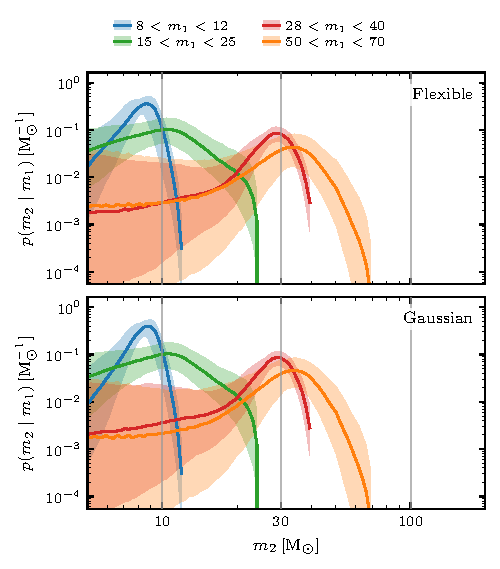
\includegraphics[width=0.6\linewidth]{draft/plots/m2_m1_windows.pdf}
    \caption{The secondary mass distribution $p(m_2 \mid m_1)$ in windows around the \featTwenty and \featSixty $\Msun$ peaks, for the \flexiblespins model. The $q \sim 0.5$ peaks map onto plateaus, not peaks, in $m_2$, because the width of their mass ratio distribution spreads a narrow peak in $m_1$ over a factor of $\sim 2$ in $m_2$. \todo{describe the bands}}
    \label{fig: m2}
\end{figure}

\todo{SM: refit $\mu$ with the $Q$ edges shifted by $\pm 0.05$ to show the locations do not depend on the band choice}


\section{The four mass features}
\label{sm: features}

\subsection{The \featTen $\Msun$ feature}

We find the global peak of the \ac{BH} mass spectrum at $m_1 = \peakTenMuFlex\,\Msun$, with a narrow width $\sigma = \peakTenSigmaFlex\,\Msun$ (Table~I of the main text).\jh{too many sig figs again} The \featTen $\Msun$ feature has been known since catalogs were a few dozens of events ~\cite[e.g.,][]{LIGOScientific:2020kqk, Talbot:2018cva, Tiwari:2020otp, Edelman:2021zkw, KAGRA:2021duu, Callister:2023tgi}, and its prominence has only grown more significant with larger catalogs \cite{LIGOScientific:2025pvj, LIGOScientific:2026ctl}. %Because it sits just above the low-mass turn-on of the \ac{BH} mass spectrum, its precise shape is partly degenerate with how that turn-on is modeled~\cite{Talbot:2018cva, LIGOScientific:2020kqk, Farah:2021qom}. 
Binaries in the \featTen $\Msun$ feature are strongly near-equal mass: in $m_1 \in [8, 12]\,\Msun$, the mode of the mass ratio distribution is $\qModeWindowTenFlex$ and its mean is $\langle q \rangle = \qWindowTenFlex$, and the feature is absent from the $q \in [0.3, 0.65]$ slice in Fig.~1 of the main text. This is consistent with~\cite{Farah:2023swu, LIGOScientific:2026ctl, Flanagan:2026ayy}, and in mild tension with some claims of a mass ratio distribution peaking away from unity at \featTen $\Msun$ \cite{Godfrey:2023oxb, Sadiq:2023zee, Sridhar:2025kvi}, and in the Isolated Peak model of \citet{LIGOScientific:2025pvj}. \todo{might want to make a plot of $p(q \mid m_1 \approx 10\,\Msun)$ for a future referee question}

The spins are small and preferentially aligned with the orbit. The mean of the effective spin distribution is $\mu_{\chieff} = \peakSpinTenEffMeanCoreFlex$ ($\peakSpinTenEffMeanCoreGauss$) in the \flexiblespins (\gaussianspins) model, positive with probability $\peakSpinTenPEffPosFlex\%$ ($\peakSpinTenPEffPosGauss\%$) and the distribution of $\chieff$ is narrow: $\sigma_{\chieff} = \peakSpinTenEffSdCoreFlex$ ($\peakSpinTenEffSdCoreGauss$). See Fig.~2 of the main text.

The precessing spins are also small. In the same region, the mean of the $\chip$ distribution is $\mu_{\chip} = \peakSpinTenPMeanFlex$ ($\peakSpinTenPMeanGauss$) and its width is $\sigma_{\chip} = \peakSpinTenPSdFlex$ ($\peakSpinTenPSdGauss$). Large in-plane spins are therefore ruled out: together with the narrow $\chieff$ distribution, this means the black holes in this feature have small spin magnitudes, not only small \textit{aligned} components. The nonzero lower bound on $\mu_{\chip}$, however, should not be taken as evidence for misaligned spins. $\chip$ is positive by construction and poorly measured for individual events, particularly for near-equal masses~\cite{Apostolatos:1994mx, Green:2020ptm}, so populations with \textit{small} vs \textit{zero} in-plane spins are remarkably difficult to distinguish~\cite[e.g.]{Vitale:2022dpa, Miller:2024sui, Vitale:2025lms}. 

% which could constrain natal kicks~\cite{Kalogera:1999tq, Gerosa:2018wbw, Callister:2020vyz}

The origin of the peak is debated. A pile-up near $10\,\Msun$ may be set when the black holes form, for example by a population of low-mass failed supernovae~\cite{Schneider:2020vvh, Schneider:2023mxe, Burrows:2024wqv, Legred:2026oiz}. Its location is then approximately fixed regardless of how the black holes are later paired, while their mass ratios are set by the pairing. Alternatively, the peak may be set by the formation channel itself: in the stable mass transfer channel, the requirement that both mass-transfer phases be stable produces a cutoff in the primary mass and a peak near $9\,\Msun$~\cite{vanSon:2022myr}. Stable mass transfer generically produces unequal masses~\cite{vanSon:2022myr, Godfrey:2026pbc}, and a pile-up near $q = 1$ arises only from systems with mass ratio reversal, where the initially less massive star forms the heavier black hole \jh{MRR papers, Floor etc.}. The near-equal masses we find are therefore in mild tension with this explanation, though the mode and mean mostly prefer a concentration towards $q\to1$, a peak as low as $q\sim 0.75$ is not ruled out (see Table~I of the main text). 

Young star clusters may also produce \ac{BBH} mergers at these masses~\cite{DiCarlo:2019pmf, Santoliquido:2020bry, Mapelli:2021gyv}, mostly from binaries that formed \textit{together} in the cluster. Near-equal masses with small, aligned spins are the expected signature of such binaries that evolved together~\cite{Zaldarriaga:2017qkw, Qin:2018vaa, Fuller:2019sxi, Bavera:2020inc, Zevin:2022wrw}, whereas binaries assembled dynamically should have isotropic spin orientations, and hence a $\chieff$ distribution symmetric about zero. We therefore take this feature to be dominated by first-generation black holes in binaries that evolved together, rather than assembled dynamically, and its near-equal masses favor a peak set at black hole formation over one set by stable mass transfer.

\subsection{The \featTwenty $\Msun$ feature}

In Fig.~1 of the main text, for mass ratios $q \in [0.3, 0.65]$, we observe a feature at $m_1\sim$ \featTwenty $\Msun$. Our Gaussian fit extracts a mean at $m_1 = \peakTwentyMuFlex\,\Msun$ with a width $\sigma = \peakTwentySigmaFlex\,\Msun$ (Table~I of the main text). Unlike the \featTen and \featThirtyFive $\Msun$ features, binaries in this feature are unequal mass: the mean mass ratio in $m_1 \in [15, 25]\,\Msun$ is $\langle q \rangle = \qWindowTwentyFlex$, and the feature does not appear in the $q \in [0.8, 1]$ slice of Fig.~1 of the main text. A joint fit to $p(m_1, q)$ with no mass ratio range imposed places the peak at $\jointTwentyMuFlex\,\Msun$, with mean mass ratio $\jointTwentyQMeanFlex$ (see the SM). Finally, within $q \in [0.3, 0.65]$, the merger rate at the peak exceeds a local power law across $m_1 \in [15, 30]\,\Msun$ with posterior probability $\peakTwentyExcessPLocFlex\%$ (c.f. $\peakTwentyExcessPLocPriorFlex\%$ prior probability). Over all mass ratios, the rate at the feature still exceeds a local power law with $P_{\rm loc} = \peakTwentyExcessPLocAllQFlex\%$.
% $\peakTwentyNEvents$ events have median $m_1 \in [15, 25]\,\Msun$ and median $q \in [0.3, 0.65]$ ($\peakTwentyNEventsPE$ by their summed posterior probability in this region).


Earlier analyses with weakly parameterized models reported hints of additional structure near $20\,\Msun$~\cite{Tiwari:2020otp, Tiwari:2021yvr, Edelman:2022ydv, Toubiana:2023egi, MaganaHernandez:2024uty}, and \citet{LIGOScientific:2025pvj} noted a possible third feature there in \ac{GWTC-4}, although the data did not require it. Using \PixelPop, \citet{LIGOScientific:2026ctl} found no evidence for such a feature in the \ac{GWTC-5} primary mass distribution. In the marginal distribution, the feature is weak because it sits between the much larger \featTen and \featThirtyFive $\Msun$ features; it becomes clearer only once the mass ratio is specified. As discussed for the \featThirtyFive $\Msun$ feature, it also fills in between the rise toward \featThirtyFive $\Msun$ in the marginal distribution. A subpopulation of rapidly spinning black holes near $16\,\Msun$ has also been proposed~\cite{Plunkett:2026pxt, Tong:2025xir, Farah:2026jlc}; the feature we find here is identified by its mass ratio, independent of the spins.


That said, the spins of binaries in this feature do differ from those at the near-equal-mass features. The effective spin distribution is broad and nearly symmetric about zero, and larger precessing spins are preferred (Fig.~2 of the main text). In the End Matter we argue that the narrow spin distribution in the \featTen and \featThirtyFive $\Msun$ features at $q\sim1$ along with the broader spins in the \featTwenty and \featSixty $\Msun$ features are $q\sim 0.5$ can explain the broadening of the $\chieff$ distribution toward unequal mass ratios~\cite{Callister:2021fpo, Adamcewicz:2023mov, LIGOScientific:2026ctl}, as argued explicitly in \citet{Vijaykumar:2026zjy}. In $m_1 \in [16, 22]\,\Msun$, $q \in [0.3, 0.65]$, $\sigma_{\chieff} = \peakSpinTwentyEffSdCoreFlex$ ($\peakSpinTwentyEffSdCoreGauss$ in the \gaussianspins model) and $\mu_{\chieff} = \peakSpinTwentyEffMeanCoreFlex$ ($\peakSpinTwentyEffMeanCoreGauss$ in the \gaussianspins model), against $\sigma_{\chieff} = \peakSpinTenEffSdCoreFlex$ and $\mu_{\chieff} = \peakSpinTenEffMeanCoreFlex$ at the \featTen $\Msun$ feature. \jh{maybe a table with all these}

\jh{averaged over primary mass, the width of the $\chieff$ distribution is $\sigma_{\chieff} = \chiQBroadSdQLoCoreFlex$ at $q = 0.35$, against $\chiQBroadSdQHiCoreFlex$ at $q = 0.85$ (Fig.~4 of the main text), consistent with the mass ratio dependence of $\chieff$ found by parametric models. }

The location, mass ratio and spins of this feature are what one qualitatively expects of second-generation mergers built from the \featTen $\Msun$ feature. Two $\sim$ \featTen $\Msun$ black holes merge into a remnant of $\sim 18\,\Msun$ with spin $\chi \approx 0.7$; if the remnant merges again with a first-generation black hole from the same peak, the binary has $q \approx 0.5$, and if it is assembled dynamically, its spins are isotropically oriented, giving a broad, symmetric $\chieff$ distribution~\cite{Fishbach:2017dwv, Gerosa:2017kvu, Rodriguez:2019huv, Gerosa:2021mno, Ginat:2026awh}. We test this quantitatively in the main text, where we find the feature sits slightly above the expected location. 

\subsection{The \featThirtyFive $\Msun$ feature}

A peak near \featThirtyFive $\Msun$ has been reported since the earliest population analyses~\cite{Talbot:2018cva, LIGOScientific:2018jsj, LIGOScientific:2020kqk, KAGRA:2021duu, Farah:2023vsc}, and more recent analyses find that the binaries in this peak prefer near-equal masses~\cite{Roy:2025ktr, Sridhar:2025kvi}. The shape of the mass spectrum at the \featThirtyFive $\Msun$ feature has previously been uncertain: \citet{LIGOScientific:2025pvj} found that the marginal primary mass distribution was consistent with either a peak \textit{or} a steepening, but could not distinguish which. Using the latest \ac{GWTC-5} dataset, \citet{LIGOScientific:2026ctl} indicated that the behavior across the \featThirtyFive $\Msun$ feature was more consistent with a steepening power law slope. 

While we observe this same ambiguity in the \textit{marginal} primary mass distribution, we emphasize that the mass spectrum for $q\in [0.8, 1]$ actually appears to prefer a \textit{peaked} \featThirtyFive $\Msun$ feature rather than the steepening of an already decreasing power law continuum: see Tab.~\ref{tab: peak odds}. The marginal merger rate in $m_1 \in [30, 35]\,\Msun$ is consistent with that in $[25, 30]\,\Msun$, but larger than that in $[35, 40]\,\Msun$ (Table~\ref{tab: peak odds}). For $q \in [0.8, 1]$, however, the merger rate rises into the $30$--$35\Msun$ window as well as falling after the window, with posterior-to-prior odds $\mathcal{O}_{\rm peak} = \peakOddsHiBFFlex$. Marginalized over all mass ratios, the odds for a localized peak drops to $\mathcal{O}_{\rm peak} = \peakOddsAllBFFlex$. The difference comes from the low-mass side of the feature: the \featTwenty $\Msun$ feature populates the region between $\featTen$ and \featThirtyFive $\Msun$ at unequal mass ratios, filling in the rise toward \featThirtyFive $\Msun$ in the marginal distribution. We argue this clarifies the degeneracy identified by \citet{LIGOScientific:2025pvj}: the steepening seen in the marginal distribution is what a near-equal-mass peak looks like once the unequal-mass binaries from the \featTwenty $\Msun$ feature are averaged in.

\begin{table}
    \renewcommand{\arraystretch}{1.3}
    \caption{Is the \featThirtyFive $\Msun$ feature a peak? We compute the odds of a rise-then-fall shape for the primary mass distribution integrated over all $q$, and the primary mass distribution restricted to $q\in[0.8,1]$. $P_{\rm peak}$ refers to the posterior probability that $R_{30\text{--}35} > R_{25\text{--}30} \,\& \, R_{25\text{--}30}$  exceeds both neighbors; $P_{\rm peak}^{\rm prior}$: the same under the prior; $\mathcal{O}_{\rm peak}$ is the implied odds ratio. The last two columns show posterior medians and 90\% intervals of ratios on merger rates in neighboring windows. Note the prior probability of $\sim \peakOddsAllPPriorFlex\%$ is smaller than the $1/3$ chance one would expect for an uncorrelated field; the Mat\'ern field prior favors monotonic behavior which \textit{a-priori} disfavors a peak in the central window. The odds for a peak are much higher in the near-equal mass ratio window, indicating a peak is statistically insignificant in the \textit{marginal} primary mass distribution, but moderately \textit{significant} for near-equal mass ratios.
}
    \label{tab: peak odds}
    \begin{ruledtabular}
    \begin{tabular}{llccccc}
        $q$ & Model & $P_{\rm peak}$ & $P_{\rm peak}^{\rm prior}$ & $\mathcal{O}_{\rm peak}$ & $\dfrac{R[{30\text{--}35}]}{R[{25\text{--}30}]}$ & $\dfrac{R[{30\text{--}35]}}{R[{35\text{--}40}]}$ \vspace{1mm} \\
        \hline
        all $q$ & \flexiblespins & $\peakOddsAllPFlex\%$ & $\peakOddsAllPPriorFlex\%$ & $\peakOddsAllBFFlex$ & $\peakOddsAllRatioLoFlex$ & $\peakOddsAllRatioHiFlex$ \\
         & \gaussianspins & $\peakOddsAllPGauss\%$ & $\peakOddsAllPPriorGauss\%$ & $\peakOddsAllBFGauss$ & $\peakOddsAllRatioLoGauss$ & $\peakOddsAllRatioHiGauss$ \\
        $[0.8, 1]$ & \flexiblespins & $\peakOddsHiPFlex\%$ & $\peakOddsHiPPriorFlex\%$ & $\peakOddsHiBFFlex$ & $\peakOddsHiRatioLoFlex$ & $\peakOddsHiRatioHiFlex$ \\
         & \gaussianspins & $\peakOddsHiPGauss\%$ & $\peakOddsHiPPriorGauss\%$ & $\peakOddsHiBFGauss$ & $\peakOddsHiRatioLoGauss$ & $\peakOddsHiRatioHiGauss$ \\
    \end{tabular}
    \end{ruledtabular}
\end{table}

\subsection{The \featSixty $\Msun$ feature}

The second unequal-mass feature is at $m_1 = \peakSixtyMuFlex\,\Msun$, with width $\sigma = \peakSixtySigmaFlex\,\Msun$ (Table~I of the main text). Like the \featTwenty $\Msun$ feature, it appears in the $q \in [0.3, 0.65]$ slice of Fig.~1 of the main text but not in the near-equal-mass slice, and the mean mass ratio in $m_1 \in [50, 70]\,\Msun$ is $\langle q \rangle = \qWindowSixtyFlex$. It is the least well measured of the four features. A joint fit to $p(m_1, q)$ with no mass ratio range imposed finds a peak in a fraction $\jointSixtyPeakFracFlex\%$ of posterior draws, at $\jointSixtyMuFlex\,\Msun$ with mean mass ratio $\jointSixtyQMeanFlex$ (SM), and within $q \in [0.3, 0.65]$ the merger rate at the peak exceeds a local power law across $m_1 \in [40, 100]\,\Msun$ with posterior probability $\peakSixtyExcessPLocFlex\%$ (c.f. $\peakSixtyExcessPLocPriorFlex\%$ prior).

Similar to the \featTwenty $\Msun$ feature, the effective spin distribution is broad and nearly symmetric (Fig.~2 of the main text), and the width of the $\chieff$ distribution grows above $\sim 45\,\Msun$, driven by the unequal-mass binaries (Fig.~5 of the main text). \red{In $m_1 \in [55, 65]\,\Msun$, $q \in [0.3, 0.65]$, $\sigma_{\chieff} = \peakSpinSixtyEffSdCoreFlex$ ($\peakSpinSixtyEffSdCoreGauss$) and $\mu_{\chieff} = \peakSpinSixtyEffMeanCoreFlex$ ($\peakSpinSixtyEffMeanCoreGauss$) (core $|\chieff| < 0.8$). The mean $\chip$, $\peakSpinSixtyPMeanFlex$ ($\peakSpinSixtyPMeanGauss$), is narrower than under the prior ($\peakSpinSixtyPMeanPriorFlex$) but centred near it, so $\chip$ is only weakly informative here.} \citet{LIGOScientific:2026ctl} similarly found a subpopulation of rapidly spinning black holes, with spins $\chi \sim 0.7$, at primary masses above $\sim 45\,\Msun$, as well as at $\sim 10$--$20\,\Msun$.

Weakly parameterized analyses of \ac{GWTC-3} and \ac{GWTC-4} showed hints of a rise in the merger rate near $60\,\Msun$~\cite{MaganaHernandez:2024uty, LIGOScientific:2025pvj}, but \citet{LIGOScientific:2026ctl} found no evidence for a peak there in the \ac{GWTC-5} primary mass distribution. They did find a flatter mass ratio distribution above $m_1 \sim 40\,\Msun$, together with the change in spin properties, and noted that this is consistent with hierarchical mergers of a second-generation and a first-generation black hole, which would have $q \approx 0.5$. Our result is in line with this, and resolves it further: the unequal-mass binaries above $\sim 40\,\Msun$ are concentrated around \featSixty $\Msun$ rather than spread across the high-mass tail. \red{Over all mass ratios, the excess at the \featSixty $\Msun$ feature has $P_{\rm loc} = \peakSixtyExcessPLocAllQFlex\%$, against $\peakSixtyExcessPLocFlex\%$ within $q \in [0.3, 0.65]$.}

A primary mass of $\sim$ \featSixty $\Msun$ lies in the pair-instability mass gap, whose lower edge has been placed near $\sim 45\,\Msun$ using the secondary masses and spins of \ac{GWTC-4} binaries~\cite{Tong:2025wpz, Antonini:2025ilj}, though see~\cite{Ray:2025xti} \todo{check these three on the location and significance of the lower edge}. Such black holes cannot form directly from stellar collapse, but can be the remnants of earlier mergers. Two $\sim$ \featThirtyFive $\Msun$ black holes merge into a remnant of $\sim 60\,\Msun$ with spin $\chi \approx 0.7$, and if this remnant merges again with a first-generation black hole from the \featThirtyFive $\Msun$ feature, the binary has $q \approx 0.5$ and, if assembled dynamically, a broad, symmetric $\chieff$ distribution~\cite{Rodriguez:2019huv, Kimball:2020opk, Gerosa:2021mno, Antonini:2024het}. Hierarchical subpopulations at high mass have also been argued for in \ac{GWTC-4}~\cite{Plunkett:2026pxt, Li:2025iux}. In the main text, we find that the location of the \featSixty $\Msun$ feature matches the remnant of the \featThirtyFive $\Msun$ feature, with $\sim 5\%$ of the mass radiated. As with the \featTwenty $\Msun$ feature, we regard the peak itself as tentative.

\section{Significance of the peaks}
\label{sm: significance}

\textit{Excess over a local power law.} For each posterior sample, we take $p(\ln m_1, q \in Q)$, the windowed mass density summed over the $q$ bins of $Q$, and in each window draw the chord in $(\ln m_1, \ln p)$ between the centers of the window's first and last bins, a local power law. The excess is
\begin{equation}
    d(m_1) = \ln p(\ln m_1, q \in Q) - \mathrm{chord}(\ln m_1),
\end{equation}
which is independent of the normalization of $p$ within $Q$, and the same for densities in $m_1$ or $\ln m_1$, since these differ by a term linear in $\ln m_1$ that the chord absorbs. We report $P_{\rm loc}$, the fraction of samples with $d > 0$ at a fixed bin, the interior bin where the median of $d$ is largest. Table~\ref{tab: excess} lists these, the height and location of the maximum excess, and the signed integrated excess $F_{\rm int} = \sum_{\rm bins}(p - e^{\rm chord}) / \sum_{\rm bins} p$. The $m_2 > 3\,\Msun$ cut removes part of the low-$m_1$ end of the window at low $q$; so that the cut cannot create a rising edge, we keep only the bins where every $q$ bin of $Q$ is allowed, i.e.\ $m_1 \min Q \geq 3\,\Msun$.

\begin{table}
    \caption{Excess over a local power law, each peak in its own mass ratio range (\flexiblespins model; medians and 90\% intervals). $P_{\rm loc}$: posterior probability of a positive excess at the most prominent bin; $d_{\max}$: the maximum excess in $\ln p$; $\hat{m}$: its location; $F_{\rm int}$: the signed integrated excess fraction.}
    \label{tab: excess}
    \begin{ruledtabular}
    \begin{tabular}{lcccc}
        Peak & $P_{\rm loc}$ & $d_{\max}$ & $\hat{m}$ [\Msun] & $F_{\rm int}$ \\
        \hline
        \featTen & $\peakTenExcessPLocFlex\%$ & $\peakTenExcessHeightFlex$ & $\peakTenExcessLocFlex$ & $\peakTenExcessFIntFlex$ \\
        \featTwenty & $\peakTwentyExcessPLocFlex\%$ & $\peakTwentyExcessHeightFlex$ & $\peakTwentyExcessLocFlex$ & $\peakTwentyExcessFIntFlex$ \\
        \featThirtyFive & $\peakThirtyFiveExcessPLocFlex\%$ & $\peakThirtyFiveExcessHeightFlex$ & $\peakThirtyFiveExcessLocFlex$ & $\peakThirtyFiveExcessFIntFlex$ \\
        \featSixty & $\peakSixtyExcessPLocFlex\%$ & $\peakSixtyExcessHeightFlex$ & $\peakSixtyExcessLocFlex$ & $\peakSixtyExcessFIntFlex$ \\
    \end{tabular}
    \end{ruledtabular}
\end{table}

\begin{figure}
    \centering
    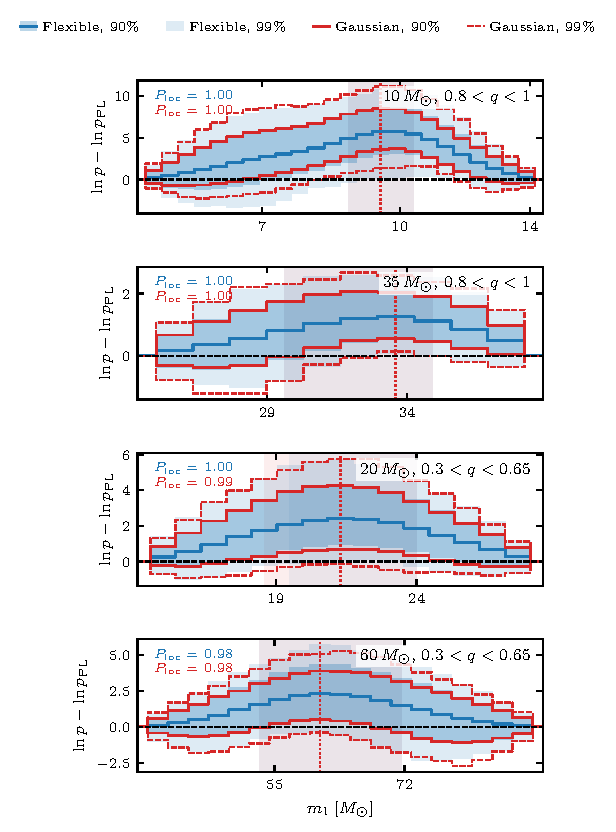
\includegraphics[width=0.6\linewidth]{draft/plots/peak_excess_own_q.pdf}
    \caption{The excess $d(m_1)$ for each peak in its own mass ratio range, per posterior sample, for the \flexiblespins (blue: 90\% and 99\% bands, median) and \gaussianspins (red: 90\% solid, 99\% dashed) models.}
    \label{fig: excess}
\end{figure}

\begin{figure}
    \centering
    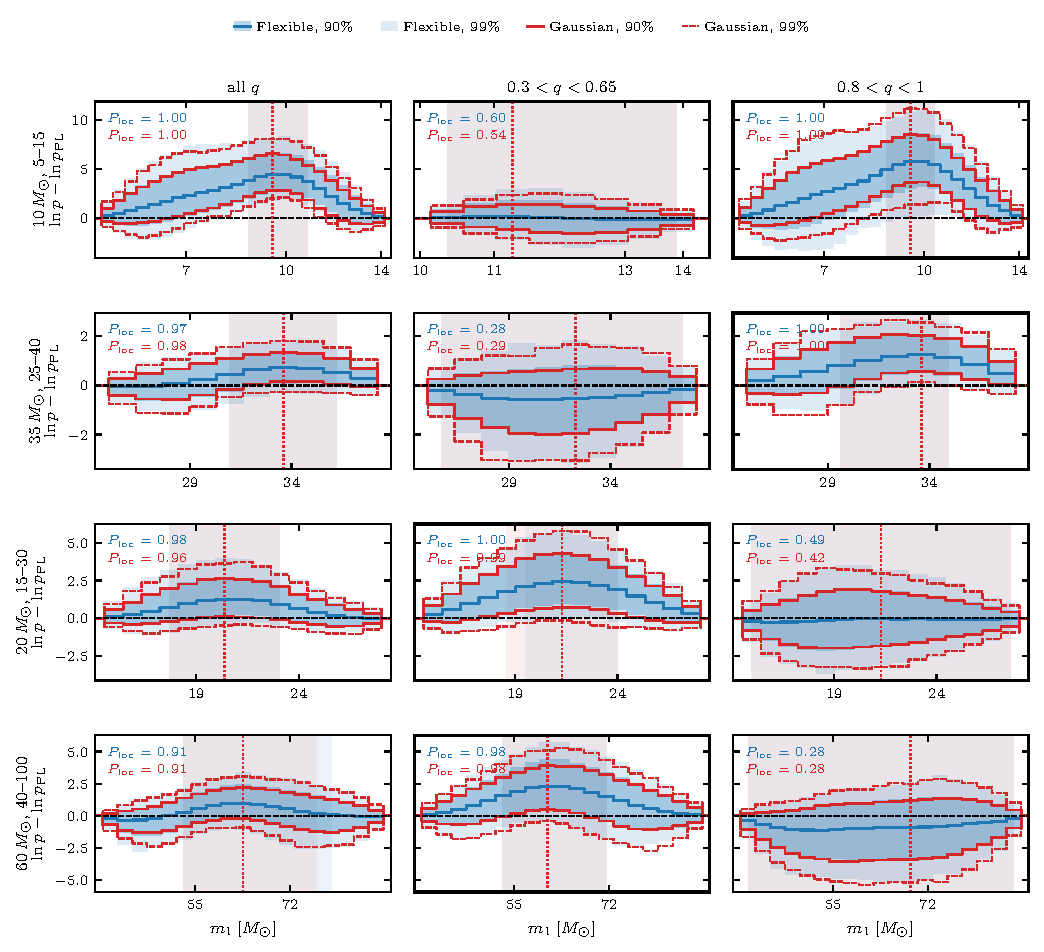
\includegraphics[width=\linewidth]{draft/plots/peak_excess.pdf}
    \caption{As Fig.~\ref{fig: excess}, for every peak window (rows) in every mass ratio range (columns: all $q$, $0.3 < q < 0.65$, $0.8 < q < 1$); boxed: each peak's own mass ratio range. The excess appears only in the boxed panels; the others show what the statistic gives without a feature.}
    \label{fig: excess grid}
\end{figure}

\textit{Mass ratio contrast.} The most direct feature in Fig.~1 of the main text and Fig.~\ref{fig: m2} is not a peak in $m_1$ but the change in the mass ratio distribution with $m_1$: near-equal masses at \featTen and \featThirtyFive $\Msun$, unequal masses at \featTwenty and \featSixty $\Msun$. In the $q \sim 0.5$ range, a peak in $p(m_1, q \in Q)$ can come entirely from the factor $P(q \in Q \mid m_1)$, so the excess above and this contrast largely measure the same feature. We test it directly with the mean mass ratio in a window $W$ around each peak,
\begin{equation}
    \langle q \rangle_W = \frac{\int_W d\ln m_1 \int_{q_0}^1 dq\, q\, p(\ln m_1, q)}{\int_W d\ln m_1 \int_{q_0}^1 dq\, p(\ln m_1, q)},
\end{equation}
with the windows of Fig.~\ref{fig: m2}: $W_{\featTen} = [8, 12]$, $W_{\featTwenty} = [15, 25]$, $W_{\featThirtyFive} = [28, 40]$ and $W_{\featSixty} = [50, 70]\,\Msun$. We take $q_0 = 0$, so the integral runs over every mass ratio the $m_2 > 3\,\Msun$ cut allows. That cut removes $q < 3\,\Msun/m_1$, that is $q \lesssim 0.25$--$0.38$ in $W_{\featTen}$ but only $q \lesssim 0.06$--$0.2$ in the other windows, so it raises $\langle q \rangle_{W_{\featTen}}$ even under the prior; we calibrate for this below. For each posterior sample we compute the contrasts
\begin{equation}
    \Delta_{\featTen,\featTwenty} = \langle q \rangle_{W_{\featTen}} - \langle q \rangle_{W_{\featTwenty}}, \quad
    \Delta_{\featThirtyFive,\featTwenty} = \langle q \rangle_{W_{\featThirtyFive}} - \langle q \rangle_{W_{\featTwenty}}, \quad
    \Delta_{\featThirtyFive,\featSixty} = \langle q \rangle_{W_{\featThirtyFive}} - \langle q \rangle_{W_{\featSixty}}.
\end{equation}
We report $P(\Delta > 0)$ and $z = \mathrm{median}(\Delta) / \sigma_\Delta$, with $\sigma_\Delta$ half the width of the central 68\% interval. Unlike $P(\Delta > 0)$ near one, $z$ does not rest on the few samples in the tail; we estimate its Monte Carlo error from the effective sample size of $\Delta$.

The contrasts improve on the chord excess in three ways:
\begin{itemize}
    \item They do not depend on where a window's ends fall.
    \item They are insensitive to a smooth curvature of $\ln p(m_1)$, which gives a positive chord excess without a peak.
    \item There are three of them, fixed by the four peaks, rather than one per window and $q$ range, and they compare the peaks with one another rather than each with its own surroundings.
\end{itemize}
The prior is stationary in $(\ln m_1, q)$, so under it $\Delta$ would be centered on zero but for the different allowed $q$ ranges, the different widths of the windows and edge effects of the grid. We therefore compute $\Delta$ under the empirical-Bayes prior draws too, and test the posterior against the prior's median $\Delta^{\rm prior}$ in place of zero: $P(\Delta > \Delta^{\rm prior})$ and $z_{\rm cal} = [\mathrm{median}(\Delta) - \Delta^{\rm prior}] / \sigma_\Delta$. The windows were still placed after inspecting the population, so these remain posterior probabilities. For the mock catalogs below, the natural statistic is the maximum of $\Delta$ over pairs of windows of a fixed width.

Table~\ref{tab: q contrast} lists the results. All three contrasts are $\approx 0.26$--$0.33$, from $\langle q \rangle = \qWindowTenFlex$ and $\qWindowThirtyFiveFlex$ at the near-equal-mass peaks and $\qWindowTwentyFlex$ and $\qWindowSixtyFlex$ at the $q \sim 0.5$ peaks (\flexiblespins; \gaussianspins: $\qWindowTenGauss$, $\qWindowThirtyFiveGauss$, $\qWindowTwentyGauss$, $\qWindowSixtyGauss$), with $z = 2.9$--$4.4$ and $P(\Delta > 0) \geq 0.99$ in both models. Under the prior, $\Delta_{\featTen,\featTwenty}$ is offset to $\approx 0.07$ ($P(\Delta > 0) \approx 0.63$) by the $m_2$ cut, and the other two contrasts are centered within $0.03$ of zero ($P \approx 0.45$--$0.56$). Against these offsets, $z_{\rm cal} = 2.6$--$4.3$ and $P(\Delta > \Delta^{\rm prior}) \geq 0.99$: the correction lowers $\Delta_{\featTen,\featTwenty}$'s significance by $\approx 1\sigma$ and leaves the others nearly unchanged. The prior's $\Delta$ is broad, $\pm 0.4$ (90\%), so a posterior $\Delta$ of $\approx 0.3$ is not unusual for a single prior draw; the test is whether the data place $\Delta$ away from the prior's center, not whether it lies outside the prior's range. Equivalently, the Bayes factor for $\Delta > 0$ against $\Delta < 0$, the posterior odds divided by the prior odds, $\mathcal{B}_{\pm} = [P/(1-P)]/[P^{\rm prior}/(1-P^{\rm prior})]$, is $\approx 80$--$300$ for \flexiblespins and $\approx 270$ to $> 1200$ for \gaussianspins. These rest on the 2--20 posterior draws with $\Delta < 0$ and are uncertain by a factor of $\gtrsim 2$; a Gaussian extrapolation of the tail would give $10^3$--$10^5$, but the posteriors of $\Delta$ have longer tails toward zero, so we quote the counts. \todo{more chains once the statistics are final, to resolve the tails} The effective sample sizes are $\approx 500$--$650$ for $\Delta_{\featTen,\featTwenty}$ and $\approx 1200$--$1500$ for the others, out of 2000 draws, so the Monte Carlo error on $P$ is $\approx 0.002$--$0.003$, comparable to $1 - P$; $z$ is the more stable measure. \todo{figure of the three posteriors}

\begin{table}
    \caption{Mass-ratio contrasts between the peaks: $\Delta$ (median and 90\% interval), $P(\Delta > 0)$, $z = \mathrm{median}(\Delta)/\sigma_\Delta$ and the effective sample size of $\Delta$, with $P(\Delta > 0)$ and $z$ under the empirical-Bayes prior, the prior's median $\Delta^{\rm prior}$, and the posterior against it, $P(\Delta > \Delta^{\rm prior})$ and $z_{\rm cal}$; $\mathcal{B}_{\pm}$, the Bayes factor for $\Delta > 0$ against $\Delta < 0$; $q_0 = 0$.}
    \label{tab: q contrast}
    \begin{ruledtabular}
    \begin{tabular}{llccccccc}
        Model & Contrast & $\Delta$ & $P(\Delta > 0)$ & $z$ & ESS & Prior $P$, $z$ & $P(\Delta > \Delta^{\rm prior})$, $z_{\rm cal}$ & $\mathcal{B}_{\pm}$ \\
        \hline
        \flexiblespins & $\Delta_{\featTen,\featTwenty}$ & $\qContrastTenTwentyMedFlex$ & $\qContrastTenTwentyPFlex\%$ & $\qContrastTenTwentyZFlex$ & $\qContrastTenTwentyESSFlex$ & $\qContrastTenTwentyPPriorFlex\%$, $\qContrastTenTwentyZPriorFlex$ & $\qContrastTenTwentyPShiftFlex\%$, $\qContrastTenTwentyZShiftFlex$ & $\qContrastTenTwentyBFFlex$ \\
        & $\Delta_{\featThirtyFive,\featTwenty}$ & $\qContrastThirtyFiveTwentyMedFlex$ & $\qContrastThirtyFiveTwentyPFlex\%$ & $\qContrastThirtyFiveTwentyZFlex$ & $\qContrastThirtyFiveTwentyESSFlex$ & $\qContrastThirtyFiveTwentyPPriorFlex\%$, $\qContrastThirtyFiveTwentyZPriorFlex$ & $\qContrastThirtyFiveTwentyPShiftFlex\%$, $\qContrastThirtyFiveTwentyZShiftFlex$ & $\qContrastThirtyFiveTwentyBFFlex$ \\
        & $\Delta_{\featThirtyFive,\featSixty}$ & $\qContrastThirtyFiveSixtyMedFlex$ & $\qContrastThirtyFiveSixtyPFlex\%$ & $\qContrastThirtyFiveSixtyZFlex$ & $\qContrastThirtyFiveSixtyESSFlex$ & $\qContrastThirtyFiveSixtyPPriorFlex\%$, $\qContrastThirtyFiveSixtyZPriorFlex$ & $\qContrastThirtyFiveSixtyPShiftFlex\%$, $\qContrastThirtyFiveSixtyZShiftFlex$ & $\qContrastThirtyFiveSixtyBFFlex$ \\
        \gaussianspins & $\Delta_{\featTen,\featTwenty}$ & $\qContrastTenTwentyMedGauss$ & $\qContrastTenTwentyPGauss\%$ & $\qContrastTenTwentyZGauss$ & $\qContrastTenTwentyESSGauss$ & $\qContrastTenTwentyPPriorGauss\%$, $\qContrastTenTwentyZPriorGauss$ & $\qContrastTenTwentyPShiftGauss\%$, $\qContrastTenTwentyZShiftGauss$ & $\qContrastTenTwentyBFGauss$ \\
        & $\Delta_{\featThirtyFive,\featTwenty}$ & $\qContrastThirtyFiveTwentyMedGauss$ & $\qContrastThirtyFiveTwentyPGauss\%$ & $\qContrastThirtyFiveTwentyZGauss$ & $\qContrastThirtyFiveTwentyESSGauss$ & $\qContrastThirtyFiveTwentyPPriorGauss\%$, $\qContrastThirtyFiveTwentyZPriorGauss$ & $\qContrastThirtyFiveTwentyPShiftGauss\%$, $\qContrastThirtyFiveTwentyZShiftGauss$ & $\qContrastThirtyFiveTwentyBFGauss$ \\
        & $\Delta_{\featThirtyFive,\featSixty}$ & $\qContrastThirtyFiveSixtyMedGauss$ & $\qContrastThirtyFiveSixtyPGauss\%$ & $\qContrastThirtyFiveSixtyZGauss$ & $\qContrastThirtyFiveSixtyESSGauss$ & $\qContrastThirtyFiveSixtyPPriorGauss\%$, $\qContrastThirtyFiveSixtyZPriorGauss$ & $\qContrastThirtyFiveSixtyPShiftGauss\%$, $\qContrastThirtyFiveSixtyZShiftGauss$ & $\qContrastThirtyFiveSixtyBFGauss$ \\
    \end{tabular}
    \end{ruledtabular}
\end{table}

\textit{What these numbers do and do not show.} We tried several measures of significance, none of which yields a calibrated $p$-value from the posterior alone:
\begin{itemize}
    \item The peak fits always find the best Gaussian in a window; on draws of the mass field's prior (empirical Bayes, as in Sec.~\ref{sm: moments}), they find a peak in 70--85\% of draws, with a median peak fraction of $\approx 0.6$. They measure where a peak is, not whether there is one.
    \item A Savage--Dickey ratio at zero peak fraction tests an exact power law, which almost no field satisfies, and is limited by the number of posterior samples.
    \item Conditional simulation of the field inside a window, given the field outside (\lq\lq inpainting''), compares the posterior with the prior's prediction. Because the kernel is fitted to the same field, the posterior realization is a typical prior draw by construction, so this test has little power.
    \item The chord excess above is positive about half the time for a featureless density with noise, and the windows were chosen after inspecting the population. It also measures curvature rather than a peak: any density whose $\ln p$ bends downward within the window, such as a steepening power law or a low-mass turn-on, gives a positive excess. The turn-on below the \featTen $\Msun$ peak contributes much of that window's excess. $P_{\rm loc}$ close to one also rests on the few samples with $d < 0$, so its Monte Carlo error is comparable to $1 - P_{\rm loc}$. \todo{effective sample size of $d$ at $m_*$}
\end{itemize}
The off-diagonal mass ratio ranges in Fig.~\ref{fig: excess grid}, where $P_{\rm loc} \approx 0.3$--$0.6$, provide a built-in reference for the last point, but not a $p$-value.

\textit{A calibrated test.} The standard is a set of mock catalogs from a null population without the feature: for example, the posterior median field with $\ln p$ in the window replaced by the chord, or by the conditional mean from outside, keeping all other features. Mock events would be drawn through the selection function, by reweighting and resampling the injections, with simulated \ac{PE} posteriors, for example Gaussian likelihoods in chirp mass, $q$ and $\chieff$ with widths calibrated on the real events. Each mock is then analyzed with exactly the same model, sampler and post-processing. The fraction of mocks with a statistic at least as large as observed is the $p$-value. Scanning the statistic over a fixed family of windows and using its maximum accounts for the look-elsewhere effect. Repeating with the feature left in measures the power. About 50--100 mocks resolve $p \sim 0.01$--$0.02$. \todo{run}

\section{Robustness and model comparisons}
\label{sm: robustness}

\textit{Spin models.} Besides the two models of the main text, we ran the \flexiblespins model with $K = 5$ instead of 10 mass modes, the \gaussianspins model with $10 \times 10$ instead of $100 \times 100$ mass modes, and the split model. The widths of $\chieff$ agree to within $\sim 0.01$ between the \gaussianspins models with 10 and 100 mass modes, so ten modes miss no structure we can resolve. All models find the broadening of $\chieff$ at $\sim 18$--$20$ and $\gtrsim 45\,\Msun$ and at low $q$; the split model finds it with lower confidence. The peak locations and mass ratios agree between all models. \todo{compare the log-likelihoods of all models} \todo{figure comparing all spin models}

\textit{Likelihood choices.} We reran both models with weaker per-event thresholds, $N_{{\rm eff}, i} \geq 50$ and $\geq 30$ (the latter for the \flexiblespins model only), and with a soft cut on the variance of the log-likelihood estimate, $\sigma^2_{\ln\mathcal{L}} < 4$ and $< 1$, imposed as a smooth penalty like the $N_{\rm eff}$ requirement. Chains with the variance cut started from the posterior sample with the smallest $\sigma^2_{\ln\mathcal{L}}$, since random prior draws, with $\sigma^2_{\ln\mathcal{L}} \sim 10^2$--$10^4$, stall against the cut. None of these changes the conclusions. The weaker $N_{\rm eff}$ thresholds and $\sigma^2_{\ln\mathcal{L}} < 4$ leave $\sigma_{\chieff}(q)$ and $\sigma_{\chieff}(m_1)$ essentially unchanged, and $P[\sigma_{\chieff}(0.85) < \sigma_{\chieff}(0.35)]$ remains 0.99--1.00 in both models. With the weaker thresholds, the \flexiblespins posterior moves to higher likelihoods with larger $\sigma^2_{\ln\mathcal{L}}$ ($\approx 6$--9), the signature of fitting Monte Carlo noise, which supports our threshold of 100. The strict cut $\sigma^2_{\ln\mathcal{L}} < 1$ softens every feature slightly, as expected from a cut that keeps the posterior away from sharp structure that the Monte Carlo integrals resolve poorly: in the \flexiblespins model, $\sigma_{\chieff}$ rises from 0.079 to 0.093 at $q = 0.85$ and falls from 0.26 to 0.23 at $q = 0.35$, and at $m_1 = 10\,\Msun$ it rises from 0.078 to 0.097. The probabilities of the width contrasts stay between 0.90 and 1.00. \todo{without the selection-bias correction}

\textit{Redshift.} To test whether the spin distribution evolves with redshift, we extended both spin models to $p(\chieff, \chip \mid m_1, q, z)$ on 10 redshift bins over $z < 1.9$, normalized in every $(m_1, q, z)$ cell: the \flexiblespins field with $10 \times 5 \times 5$ modes in $(\ln m_1, q, z)$, and the \gaussianspins parameter fields with $100 \times 100 \times 10$ modes. Both models give the same picture. At fixed low $q$, $\sigma_{\chieff}$ does not change with redshift. Near equal masses it grows from $\approx 0.06$--$0.07$ at $z \approx 0.1$ to $\approx 0.11$--$0.13$ at $z \approx 0.9$, with probability $\approx 0.9$ in every primary-mass range, and the mean of $\chip$ grows from $\approx 0.2$ to $\approx 0.3$. We do not regard these trends as measurements. The detected \acp{BBH} at $m_1 \lesssim 25\,\Msun$ lie almost entirely at $z \lesssim 0.4$, while those at $z \gtrsim 0.5$ are heavier, so the field must join narrow $\chieff$ at low mass and low redshift to the broader $\chieff$ at high mass and high redshift, and can only do so in the region without data, at low mass and high redshift. At higher redshift, mass ratios and $\chip$ are also less well measured, so the moments revert toward each model's default. To remove the first effect, we also fit a \gaussianspins model in which each parameter is $\theta_i = c_i + f_i(\ln m_1, q) + g_i(z)$, with $g_i$ a one-dimensional Mat\'ern field on 100 redshift modes, shared by all $(m_1, q)$ and with its own amplitude, smoothness and range; its constant mode is set to zero, like that of $f_i$. A redshift trend in this model must appear wherever the data reach. \todo{results of the additive model: posterior of the amplitudes of $g_i$ against their prior}

\textit{Influential events.} \todo{leave-one-out on the events that dominate each $q \sim 0.5$ window, including GW231123; split by observing run}

\textit{Core threshold.} \todo{$\sigma_{\chieff}(q)$ for $|\chieff| < 0.6$, 0.7, 0.9 and without restriction}

\textit{Single-variable spin models.} Figure~\ref{fig: single} compares the \gaussianspins model with a joint field $F(\ln m_1, q)$ against the additive $F_{\ln m_1} + F_q$ model of the End Matter and the two single-variable models, $F_q$ only and $F_{\ln m_1}$ only.

\textit{Mass ratio dependence of} $\chip$\textit{.} The dependence of $\chip$ on mass ratio is less robust than that of $\chieff$. In the \flexiblespins model, the mean and width of $\chip$ both decrease toward $q = 1$, with the width falling from $\sim 0.2$ at $q \lesssim 0.5$ to $\sim 0.1$ near $q = 1$, mirroring the narrowing of $\chieff$ (Fig.~4 of the main text); in the \gaussianspins model, both are nearly independent of $q$. We therefore do not claim a mass ratio dependence of $\chip$. Finally, as for the \featTen $\Msun$ feature, we do not interpret the nonzero lower bounds on the mean of $\chip$ as evidence for misaligned spins, since $\chip$ is positive by construction and poorly measured for individual events~\cite{Vitale:2022dpa, Miller:2024sui}. \todo{add \texttt{chi\_p\_mean\_sd\_m1\_prior.pdf} and \texttt{chi\_p\_mean\_sd\_q\_prior.pdf} to the SM}

\textit{Redshift and selection.} A similar argument applies to redshift. At fixed $m_1$ and $q$, the width is constant in redshift (Fig.~6 of the main text, top right), and within each band of mass ratio it stays at $\sim 0.07$ for $q \in [0.8, 1]$ and $\sim 0.2$ for $q \in [0.3, 0.65]$ out to $z \approx 1.9$. The broadening with redshift found in earlier work~\cite{Biscoveanu:2022qac} can arise from selection effects. Heavier binaries are detectable farther away, so the mean detected primary mass grows from $\sim 13\,\Msun$ at $z \approx 0.05$ to $\sim 40\,\Msun$ by $z \approx 1$. As a result, the $\chieff$ width of the detectable binaries in our population increases by a factor $\sim 1.6$ over that range, even though the population width does not \red{(Fig.~\ref{fig: sigma obs})}. A spin model that depends on redshift alone, fit with a selection correction that does not depend on spin, would recover approximately this detected width.

\begin{figure}
    \centering
    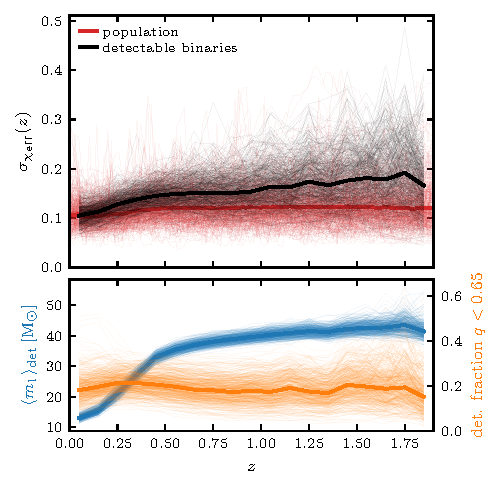
\includegraphics[width=\linewidth]{draft/plots/chi_eff_sd_z_observed_traces.pdf}
    \caption{\red{Draft caption. Selection makes a redshift trend in the detected spins without one in the population. Top: the width of the $\chieff$ distribution against redshift, for the population (red) and for the binaries detectable in it (black), in the additive \gaussianspins model; 500 posterior draws (thin) and their medians (thick), the same draws in both. The detectable width uses each draw's own weights on the found injections, the same weights as in the selection term. Bottom: the mean primary mass of detectable binaries (blue, left axis), and the fraction with $q < 0.65$ (orange, right axis). The population width is flat, but the detectable width grows by a factor $\sim 1.6$ out to $z \approx 1.3$ as the detected sample shifts from the $\sim$ \featTen $\Msun$ peak to heavier binaries; the unequal-mass fraction stays at $\sim 0.2$. Above $z \approx 1.2$ the detectable curves are noisy, with only a few hundred effective injections per redshift bin. (\texttt{plots/chi\_eff\_sd\_z\_observed\_traces.pdf}, one column.)}}
    \label{fig: sigma obs}
\end{figure}

\begin{figure*}
    \centering
    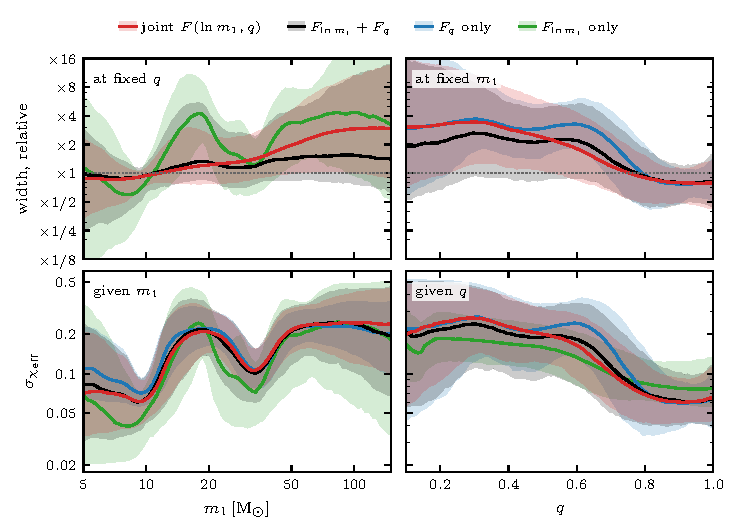
\includegraphics[width=0.75\linewidth]{draft/plots/chi_eff_sd_conditional_marginal_single.pdf}
    \caption{\red{Draft caption. As Fig.~6 of the main text, without redshift dependence, for the \gaussianspins model with a joint field $F(\ln m_1, q)$ (red) and three additive ones: $F_{\ln m_1} + F_q$ (black), $F_q$ only (blue) and $F_{\ln m_1}$ only (green). Top: the conditional width at fixed $q$ (left) and at fixed $m_1$ (right), relative to the population average; a model without that dependence is not shown. For the joint model, which is not separable, this is the partial dependence: $\ln \sigma$ averaged over the population $p(q)$ at each $m_1$ (left) and over $p(m_1)$ at each $q$ (right), which for an additive model is $F_{\ln m_1}$ ($F_q$) up to a constant. Bottom: the marginals $\sigma_{\chieff}$ given $m_1$ and given $q$. Median and 90\%. Either variable alone reproduces much of the marginal structure in the other: the $F_q$-only model recovers the narrow--broad--narrow--broad $\sigma_{\chieff}(m_1)$, and the $F_{\ln m_1}$-only model, which needs explicit structure in $m_1$ to do so, gives a broadening of $\sigma_{\chieff}(q)$ toward low $q$ that is more gradual than the sharp drop near $q \approx 0.7$ of the other two. When both are allowed, the dependence is placed on $q$.}}
    \label{fig: single}
\end{figure*}

\section{Hierarchical-merger expectations}
\label{sm: hierarchical}

\textit{Remnant mass and spin.} A merger of two non-spinning \acp{BH} with mass ratio near one radiates $\approx 5\%$ of its total mass in gravitational waves and leaves a remnant with dimensionless spin $\chi_f \approx 0.69$; both depend weakly on mass ratio and on the component spins~\cite{Gerosa:2021mno}. The second-generation peak should therefore sit at $\approx 0.95\,\mu_{\rm lo}(1 + \langle q \rangle_{\rm lo})$, and its remnant spins should be large.

\textit{Effective spins.} In a dense cluster, the second-generation \ac{BH} pairs dynamically with a first-generation companion, and its spin is isotropically oriented relative to the new orbit. With primary spin $\chi_1 = \chi_f$ at tilt $\theta_1$ and a slowly spinning secondary,
\begin{equation}
    \chieff \approx \frac{\chi_f \cos\theta_1}{1 + q}, \qquad \chip \approx \chi_f \sin\theta_1.
\end{equation}
For isotropic tilts, $\langle\cos\theta\rangle = 0$, $\langle\cos^2\theta\rangle = 1/3$, $\langle\sin\theta\rangle = \pi/4$ and $\langle\sin^2\theta\rangle = 2/3$, so at $q = 0.5$
\begin{equation}
    \langle\chieff\rangle = 0, \quad \sigma_{\chieff} = \frac{\chi_f}{(1+q)\sqrt{3}} \approx 0.27, \quad \langle\chip\rangle = \frac{\pi}{4}\chi_f \approx 0.54, \quad \sigma_{\chip} = \chi_f\sqrt{\frac{2}{3} - \frac{\pi^2}{16}} \approx 0.15.
\end{equation}
Including the secondary's term in $\chip = \max[\chi_1\sin\theta_1, \frac{3 + 4q}{4 + 3q} q\, \chi_2\sin\theta_2]$, with $\chi_2 \sim 0.1$--$0.2$, raises $\langle\chip\rangle$ by $\approx 0.01$--$0.02$. The distribution of $\chip$ is concentrated near $\chi_f$, since $\sin\theta$ is close to one over most of the sphere, and $\chieff$ and $\chip$ are uncorrelated but strongly dependent, lying near the arc $(1+q)^2\chieff^2 + \chip^2 \approx \chi_f^2$.

\textit{Mixtures.} The window around a $q \sim 0.5$ peak also contains first-generation binaries. If a fraction $f$ of the window is second-generation, the expected moments are
\begin{equation}
    \langle\chieff\rangle = (1 - f)\langle\chieff\rangle_{\rm 1G}, \qquad \sigma^2_{\chieff} = f\,\sigma^2_{\rm 2G} + (1 - f)\,\sigma^2_{\rm 1G} + f(1 - f)\,\langle\chieff\rangle_{\rm 1G}^2,
\end{equation}
and similarly for $\chip$. The peak fractions of the window fits give $f$, and the near-equal-mass peaks give the first-generation moments, so this prediction has no free parameters. \todo{evaluate}

\textit{Alternatives.} Hierarchical mergers in active galactic nuclei disks would instead produce preferentially aligned spins, and so positive $\chieff$ at low mass ratio~\cite{Li:2025iux}. The mean of $\chieff$ in our models is nearly independent of $q$ while its width grows, which favors isotropic orientations. \todo{quote $P(\mu_{\chieff} > 0)$ at the \featTwenty and \featSixty $\Msun$ peaks}

\section{Additional figures}

\begin{figure}
    \centering
    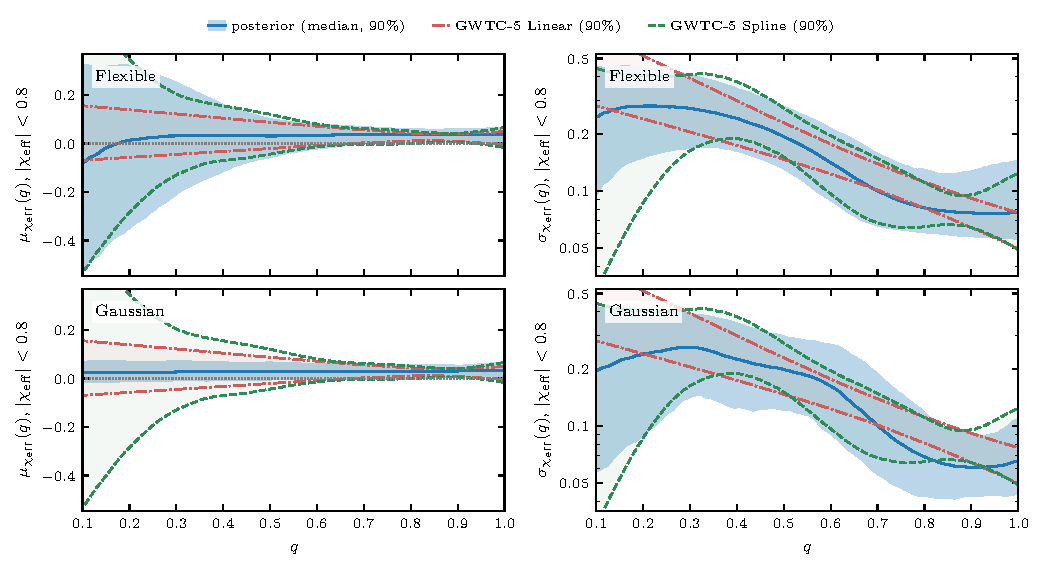
\includegraphics[width=\linewidth]{draft/plots/chi_eff_mean_sd_q_core_lvk.pdf}
    \caption{The mean (left) and width (right) of $\chieff$ as a function of mass ratio, as in Fig.~4 of the main text, with the GWTC-5 linear and spline $\chieff \mid q$ models.}
    \label{fig: mean width q}
\end{figure}

\begin{figure}
    \centering
    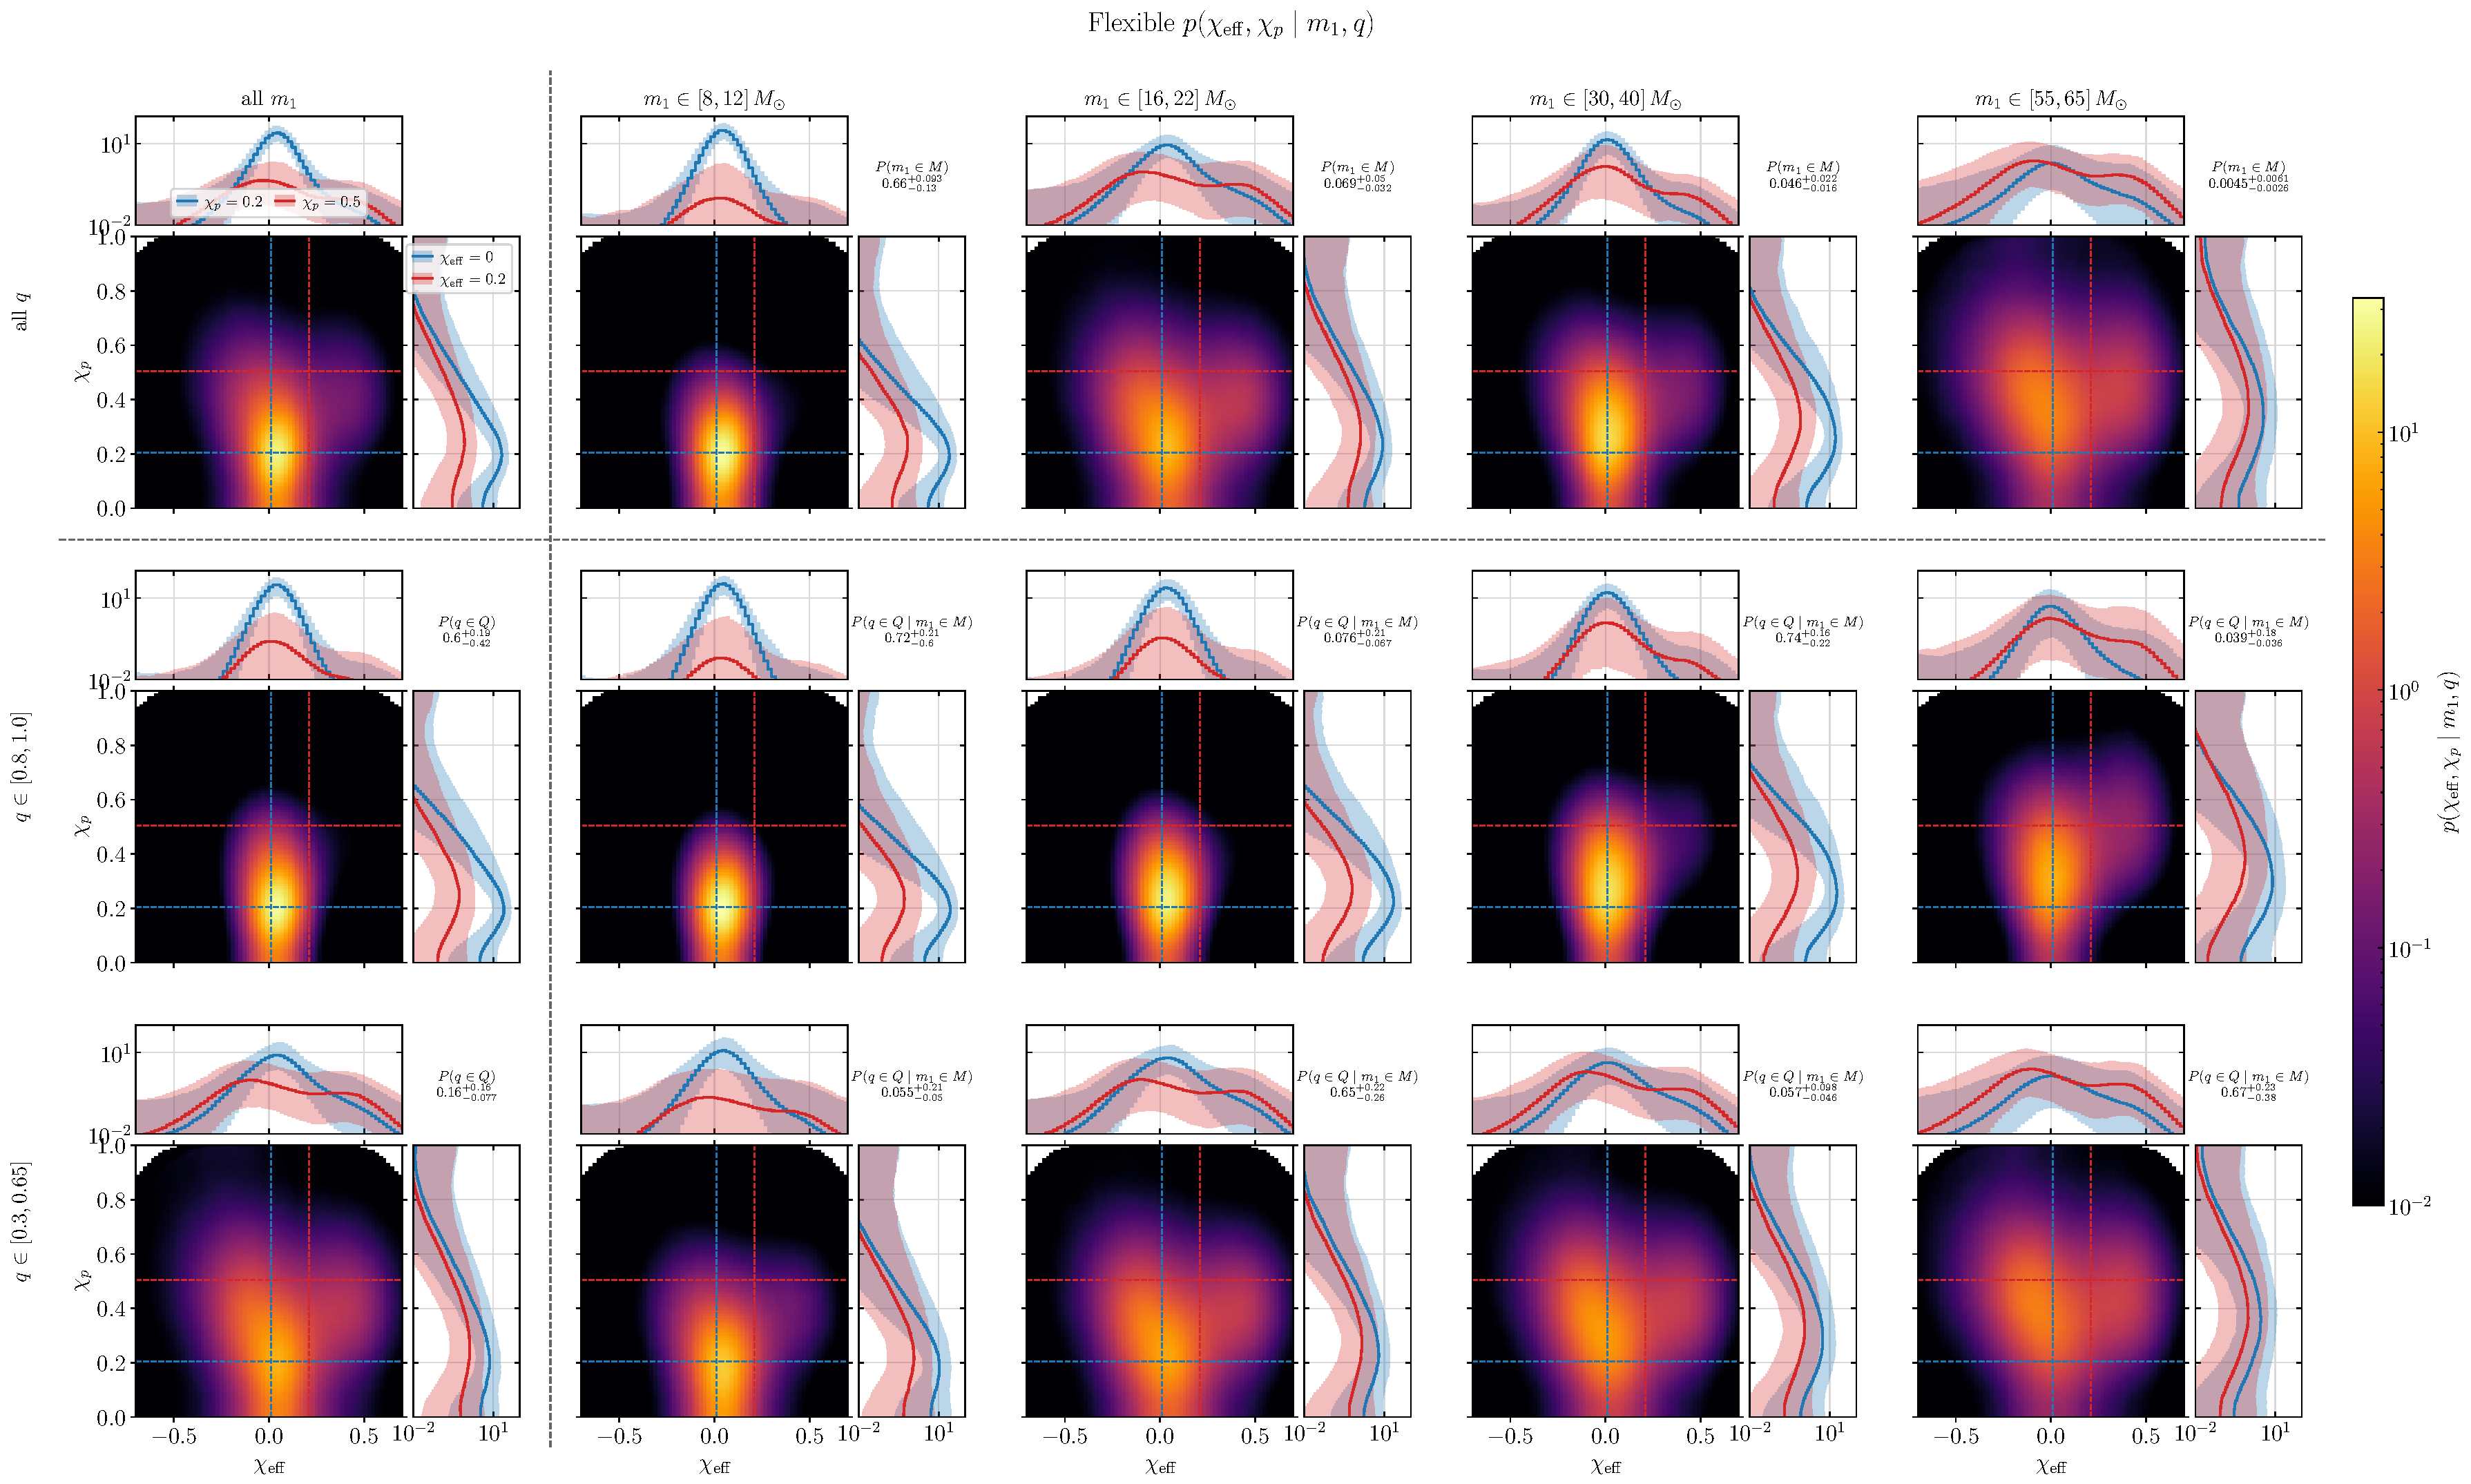
\includegraphics[width=\linewidth]{draft/plots/spin_regions_flexible.pdf}
    \caption{The joint spin distribution across the $(m_1, q)$ plane for the \flexiblespins model. \todo{caption}}
    \label{fig: regions flexible}
\end{figure}

\begin{figure}
    \centering
    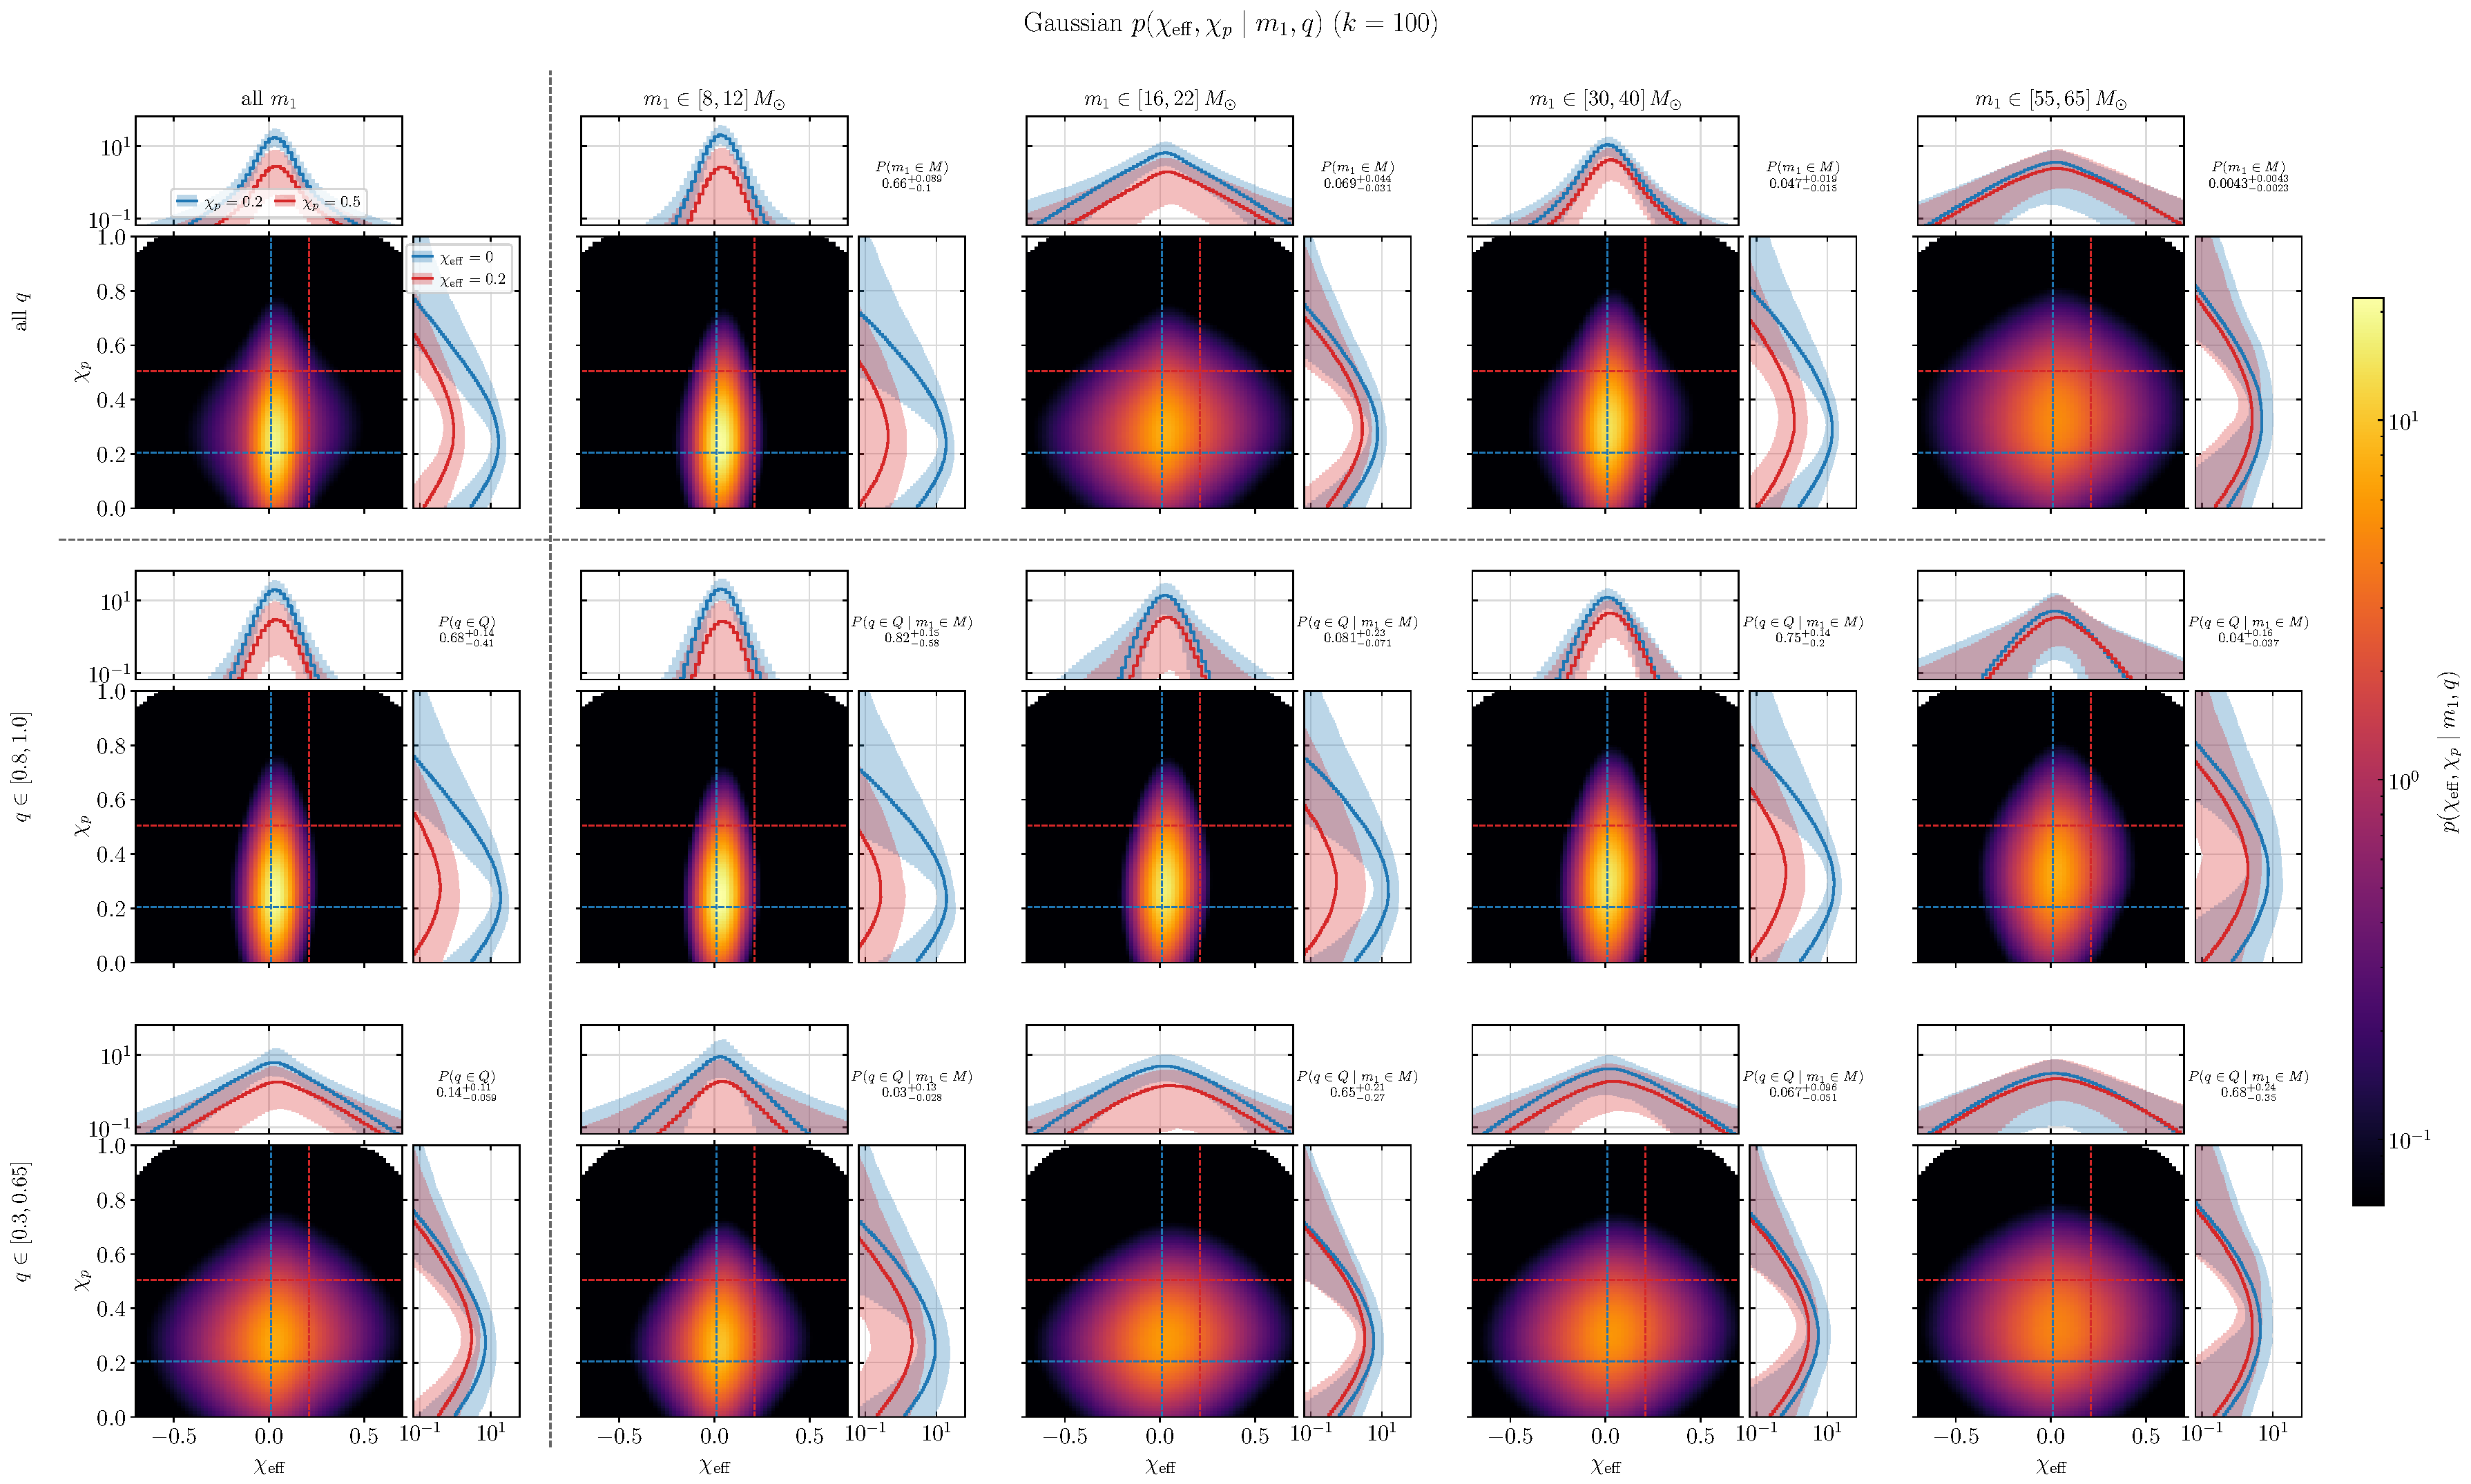
\includegraphics[width=\linewidth]{draft/plots/spin_regions_gaussian.pdf}
    \caption{As Fig.~\ref{fig: regions flexible}, for the \gaussianspins model.}
    \label{fig: regions gaussian}
\end{figure}

\begin{figure*}
    \centering
    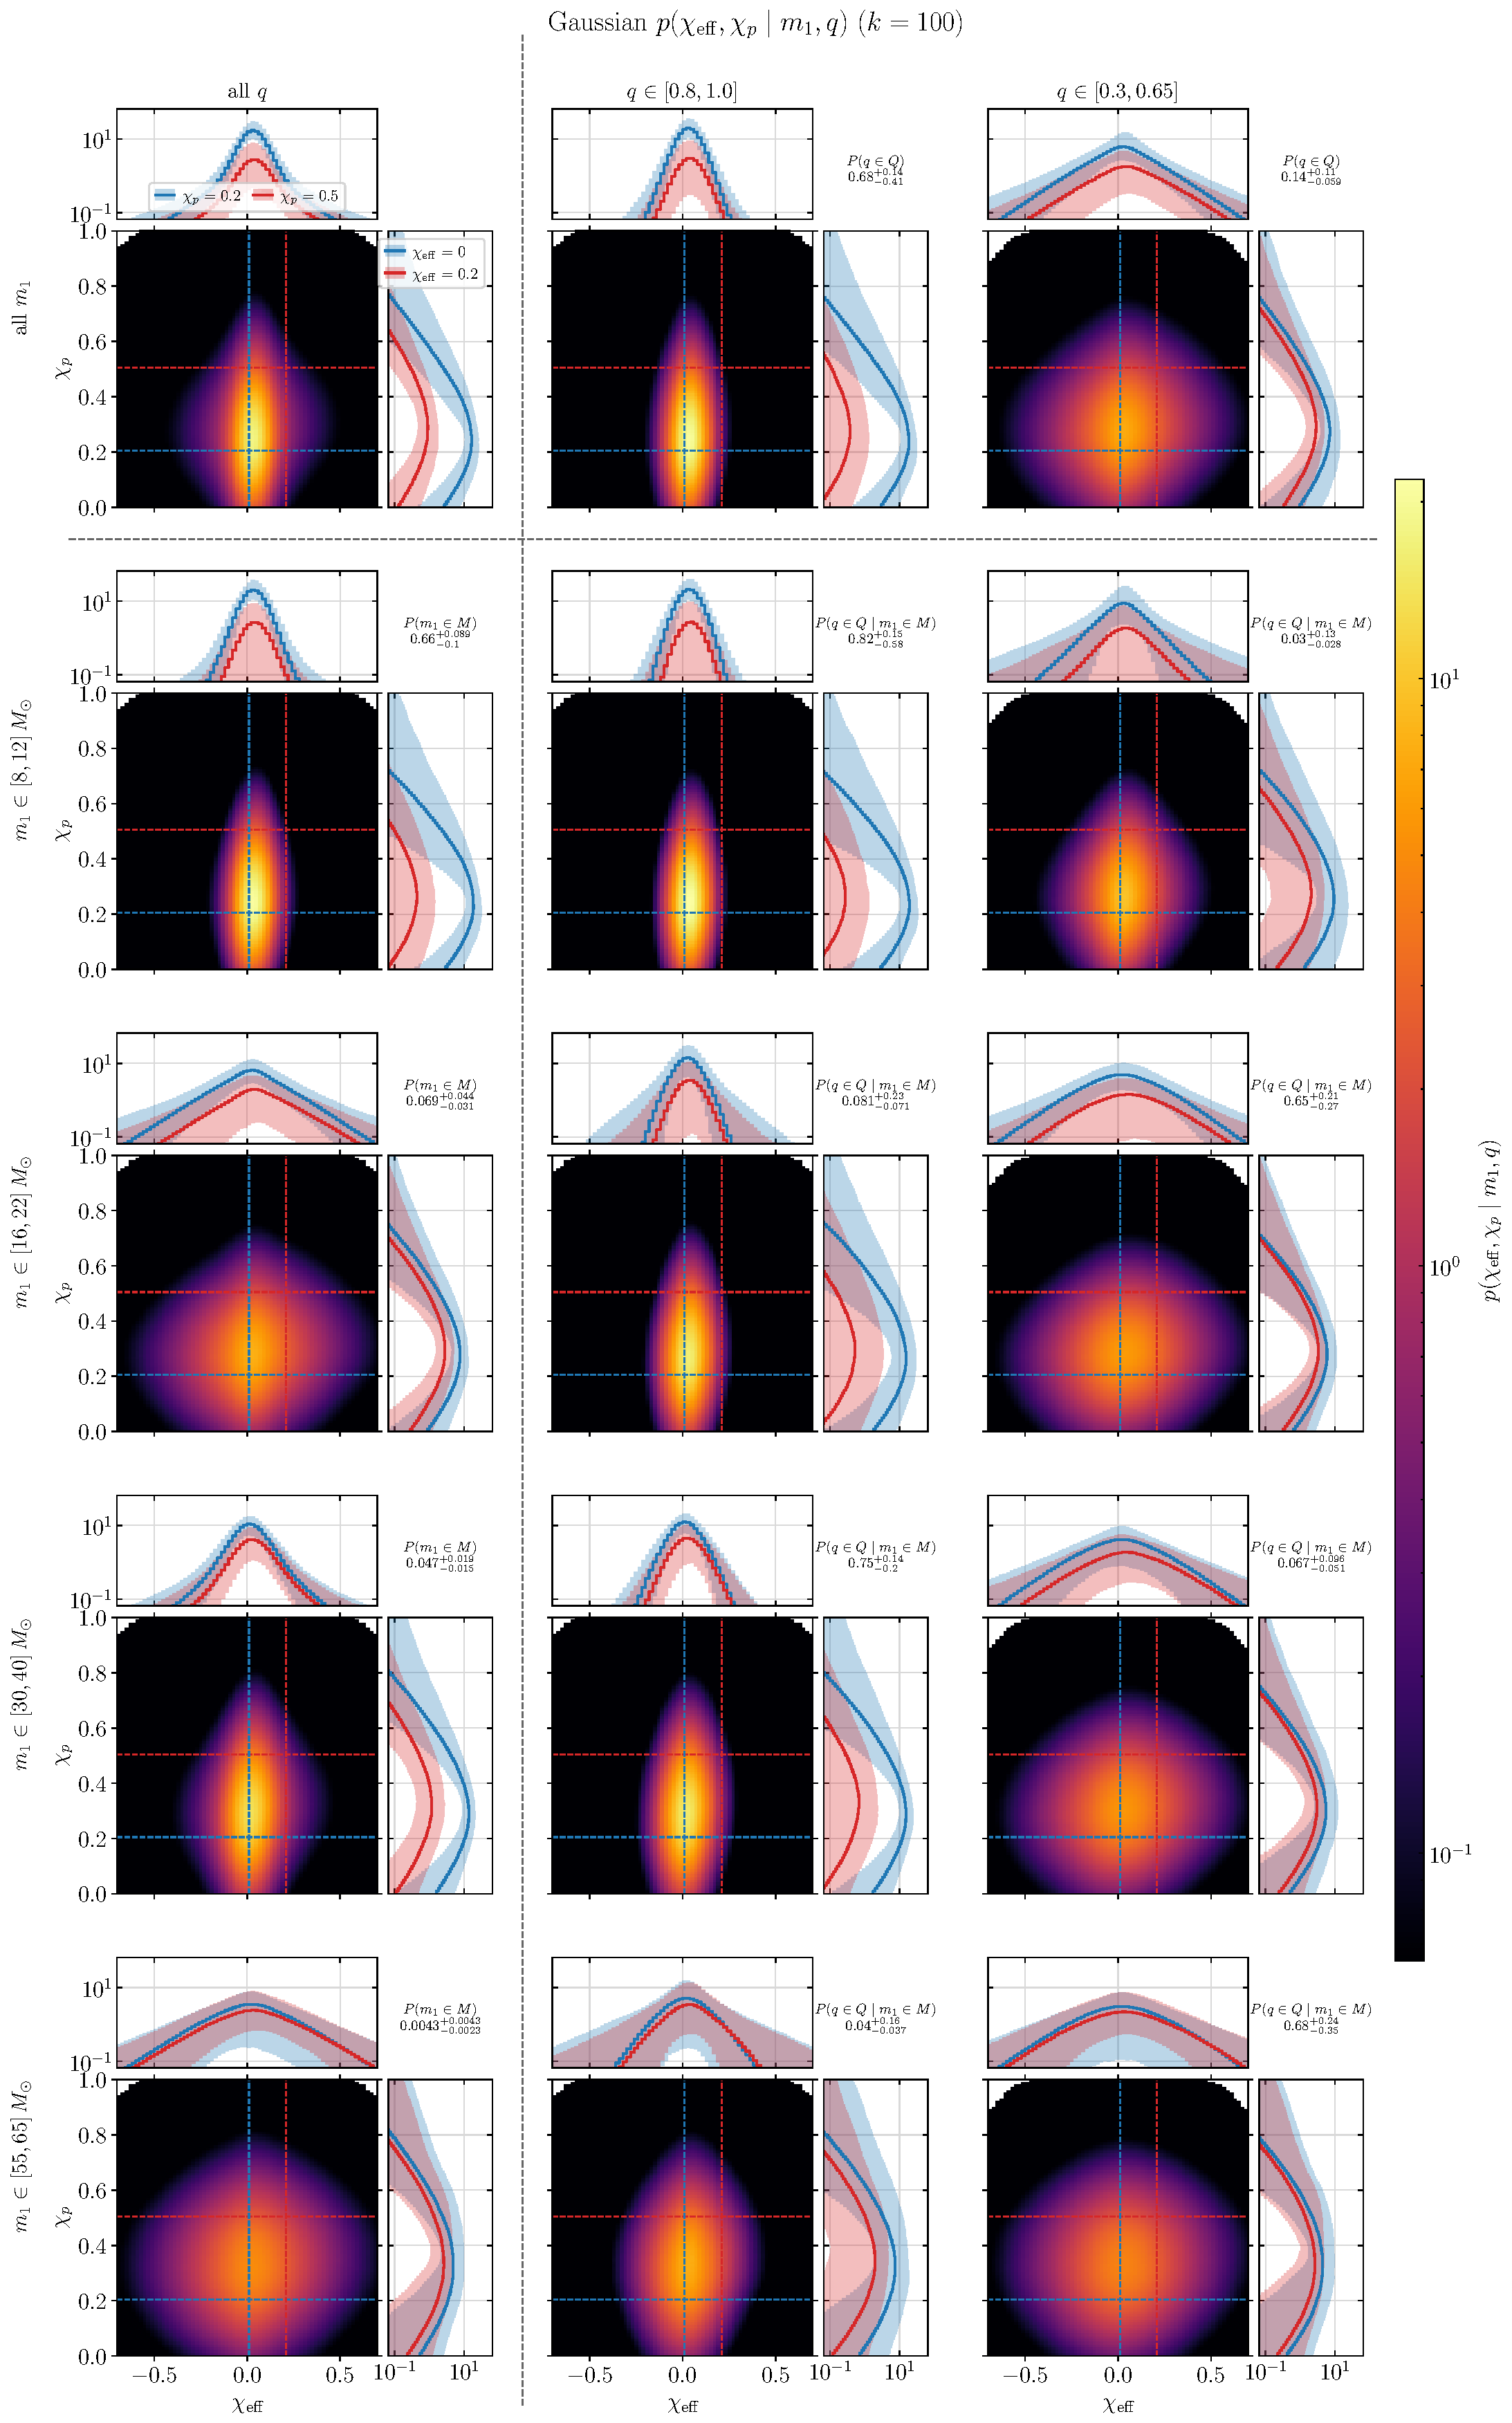
\includegraphics[height=\textheight]{draft/plots/spin_regions_gaussian_T.pdf}
    \caption{\red{Move to the SM: full spin-region grid for the Gaussian model.}}
    \label{fig:placeholder}
\end{figure*}


\bibliography{draft/main}

\end{document}
